\documentclass[10pt]{article}
\usepackage[a4paper,margin=1.5cm]{geometry}
\usepackage[compat=1.1.0]{tikz-feynman}
\tikzfeynmanset{warn luatex=false, every vertex={font=\small}}
\begin{document}
\section*{Triple-real channels: one representative diagram each}
QGRAF diagrams (all legs incoming); initial state $p_1, p_2$ on the left, $V$ and the final state $r_1, r_2, r_3$ on the right (final-state particles = conjugates of the QGRAF fields). Representative: first diagram with only 3-point vertices and $V$ on the $q$ line. Black: $q$, blue: $Q$, dotted: ghosts, curly: gluons, wavy: $V$. Arrows: fermion flow.\par\medskip
\section*{\texttt{physical\_qqbggg}}
\begin{minipage}[t]{0.48\textwidth}\centering\resizebox{0.95\linewidth}{!}{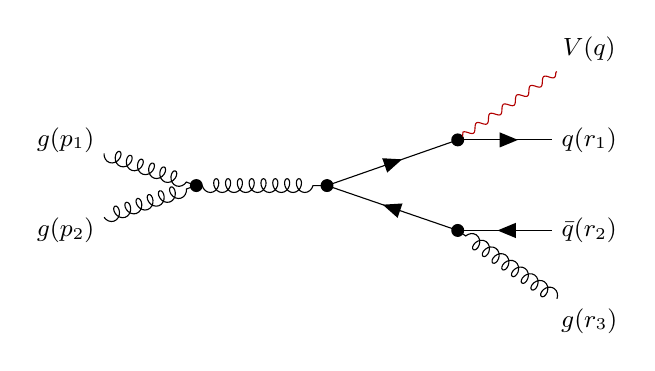
\begin{tikzpicture}[baseline=(current bounding box.center)]
\begin{feynman}
\vertex (e1) at (0.43,2.59) {\small $g(p_1)$};
\vertex (e3) at (0.43,1.44) {\small $g(p_2)$};
\vertex (e5) at (7.08,3.74) {\small $V(q)$};
\vertex (e7) at (7.08,2.59) {\small $q(r_1)$};
\vertex (e9) at (7.08,1.44) {\small $\bar q(r_2)$};
\vertex (e11) at (7.08,0.29) {\small $g(r_3)$};
\vertex[dot] (v0) at (2.09,2.01) {};
\vertex[dot] (v1) at (5.41,2.59) {};
\vertex[dot] (v2) at (5.41,1.44) {};
\vertex[dot] (v3) at (3.75,2.01) {};
\diagram* {
(e1) -- [gluon] (v0),
(e3) -- [gluon] (v0),
(e5) -- [boson, red!70!black] (v1),
(v1) -- [fermion] (e7),
(e9) -- [fermion] (v2),
(e11) -- [gluon] (v2),
(v0) -- [gluon] (v3),
(v3) -- [fermion] (v1),
(v2) -- [fermion] (v3),
};
\end{feynman}
\end{tikzpicture}}\\[2mm]\textbf{Vggqqbg}: $g g \to V\, q \bar q g$\\ {\footnotesize diagram 3 of 50, p1$\leftrightarrow$p2 symmetric}\end{minipage}\hfill%
\begin{minipage}[t]{0.48\textwidth}\centering\resizebox{0.95\linewidth}{!}{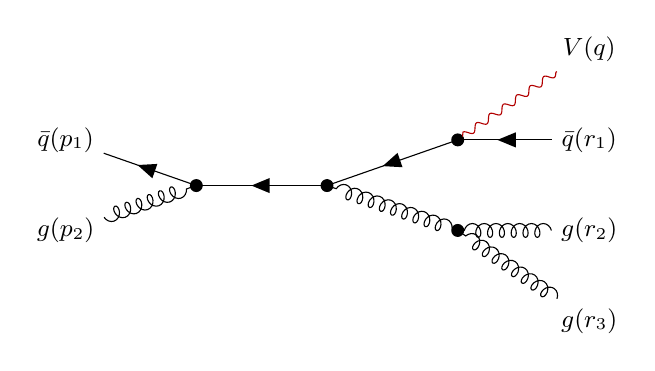
\begin{tikzpicture}[baseline=(current bounding box.center)]
\begin{feynman}
\vertex (e1) at (0.43,2.59) {\small $\bar q(p_1)$};
\vertex (e3) at (0.43,1.44) {\small $g(p_2)$};
\vertex (e5) at (7.08,3.74) {\small $V(q)$};
\vertex (e7) at (7.08,2.59) {\small $\bar q(r_1)$};
\vertex (e9) at (7.08,1.44) {\small $g(r_2)$};
\vertex (e11) at (7.08,0.29) {\small $g(r_3)$};
\vertex[dot] (v0) at (2.09,2.01) {};
\vertex[dot] (v1) at (5.41,2.59) {};
\vertex[dot] (v2) at (5.41,1.44) {};
\vertex[dot] (v3) at (3.75,2.01) {};
\diagram* {
(v0) -- [fermion] (e1),
(e3) -- [gluon] (v0),
(e5) -- [boson, red!70!black] (v1),
(e7) -- [fermion] (v1),
(e9) -- [gluon] (v2),
(e11) -- [gluon] (v2),
(v3) -- [fermion] (v0),
(v1) -- [fermion] (v3),
(v2) -- [gluon] (v3),
};
\end{feynman}
\end{tikzpicture}}\\[2mm]\textbf{Vqbgqbgg}: $\bar q g \to V\, \bar q g g$\\ {\footnotesize diagram 3 of 50, p1$\leftrightarrow$p2 partner Vgqbqbgg}\end{minipage}\hfill

\bigskip

\begin{minipage}[t]{0.48\textwidth}\centering\resizebox{0.95\linewidth}{!}{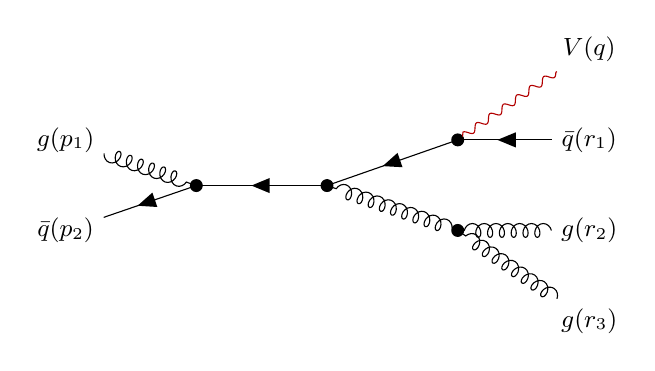
\begin{tikzpicture}[baseline=(current bounding box.center)]
\begin{feynman}
\vertex (e1) at (0.43,2.59) {\small $g(p_1)$};
\vertex (e3) at (0.43,1.44) {\small $\bar q(p_2)$};
\vertex (e5) at (7.08,3.74) {\small $V(q)$};
\vertex (e7) at (7.08,2.59) {\small $\bar q(r_1)$};
\vertex (e9) at (7.08,1.44) {\small $g(r_2)$};
\vertex (e11) at (7.08,0.29) {\small $g(r_3)$};
\vertex[dot] (v0) at (2.09,2.01) {};
\vertex[dot] (v1) at (5.41,2.59) {};
\vertex[dot] (v2) at (5.41,1.44) {};
\vertex[dot] (v3) at (3.75,2.01) {};
\diagram* {
(e1) -- [gluon] (v0),
(v0) -- [fermion] (e3),
(e5) -- [boson, red!70!black] (v1),
(e7) -- [fermion] (v1),
(e9) -- [gluon] (v2),
(e11) -- [gluon] (v2),
(v3) -- [fermion] (v0),
(v1) -- [fermion] (v3),
(v2) -- [gluon] (v3),
};
\end{feynman}
\end{tikzpicture}}\\[2mm]\textbf{Vgqbqbgg}: $g \bar q \to V\, \bar q g g$\\ {\footnotesize diagram 3 of 50, p1$\leftrightarrow$p2 partner Vqbgqbgg}\end{minipage}\hfill%
\begin{minipage}[t]{0.48\textwidth}\centering\resizebox{0.95\linewidth}{!}{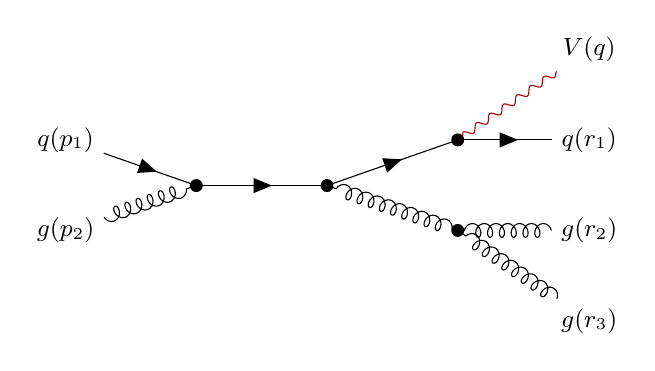
\begin{tikzpicture}[baseline=(current bounding box.center)]
\begin{feynman}
\vertex (e1) at (0.43,2.59) {\small $q(p_1)$};
\vertex (e3) at (0.43,1.44) {\small $g(p_2)$};
\vertex (e5) at (7.08,3.74) {\small $V(q)$};
\vertex (e7) at (7.08,2.59) {\small $q(r_1)$};
\vertex (e9) at (7.08,1.44) {\small $g(r_2)$};
\vertex (e11) at (7.08,0.29) {\small $g(r_3)$};
\vertex[dot] (v0) at (2.09,2.01) {};
\vertex[dot] (v1) at (5.41,2.59) {};
\vertex[dot] (v2) at (5.41,1.44) {};
\vertex[dot] (v3) at (3.75,2.01) {};
\diagram* {
(e1) -- [fermion] (v0),
(e3) -- [gluon] (v0),
(e5) -- [boson, red!70!black] (v1),
(v1) -- [fermion] (e7),
(e9) -- [gluon] (v2),
(e11) -- [gluon] (v2),
(v0) -- [fermion] (v3),
(v3) -- [fermion] (v1),
(v2) -- [gluon] (v3),
};
\end{feynman}
\end{tikzpicture}}\\[2mm]\textbf{Vqgqgg}: $q g \to V\, q g g$\\ {\footnotesize diagram 3 of 50, p1$\leftrightarrow$p2 partner Vgqqgg}\end{minipage}\hfill

\bigskip

\begin{minipage}[t]{0.48\textwidth}\centering\resizebox{0.95\linewidth}{!}{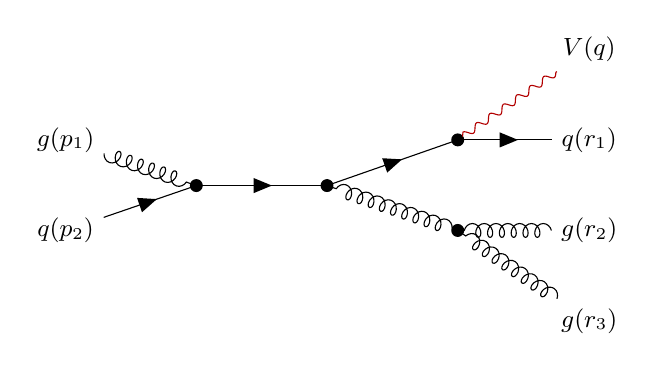
\begin{tikzpicture}[baseline=(current bounding box.center)]
\begin{feynman}
\vertex (e1) at (0.43,2.59) {\small $g(p_1)$};
\vertex (e3) at (0.43,1.44) {\small $q(p_2)$};
\vertex (e5) at (7.08,3.74) {\small $V(q)$};
\vertex (e7) at (7.08,2.59) {\small $q(r_1)$};
\vertex (e9) at (7.08,1.44) {\small $g(r_2)$};
\vertex (e11) at (7.08,0.29) {\small $g(r_3)$};
\vertex[dot] (v0) at (2.09,2.01) {};
\vertex[dot] (v1) at (5.41,2.59) {};
\vertex[dot] (v2) at (5.41,1.44) {};
\vertex[dot] (v3) at (3.75,2.01) {};
\diagram* {
(e1) -- [gluon] (v0),
(e3) -- [fermion] (v0),
(e5) -- [boson, red!70!black] (v1),
(v1) -- [fermion] (e7),
(e9) -- [gluon] (v2),
(e11) -- [gluon] (v2),
(v0) -- [fermion] (v3),
(v3) -- [fermion] (v1),
(v2) -- [gluon] (v3),
};
\end{feynman}
\end{tikzpicture}}\\[2mm]\textbf{Vgqqgg}: $g q \to V\, q g g$\\ {\footnotesize diagram 3 of 50, p1$\leftrightarrow$p2 partner Vqgqgg}\end{minipage}\hfill%
\begin{minipage}[t]{0.48\textwidth}\centering\resizebox{0.95\linewidth}{!}{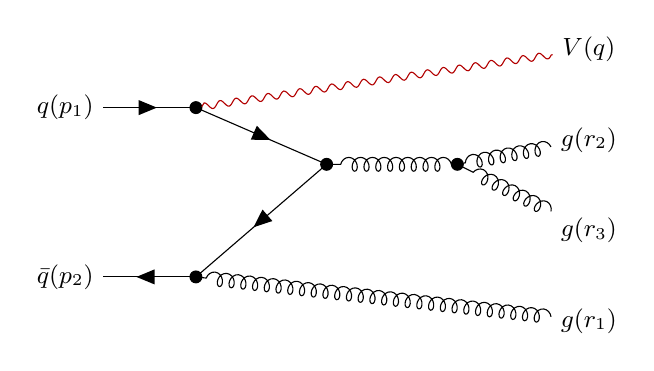
\begin{tikzpicture}[baseline=(current bounding box.center)]
\begin{feynman}
\vertex (e1) at (0.43,3.00) {\small $q(p_1)$};
\vertex (e3) at (0.43,0.85) {\small $\bar q(p_2)$};
\vertex (e5) at (7.08,3.74) {\small $V(q)$};
\vertex (e7) at (7.08,0.29) {\small $g(r_1)$};
\vertex (e9) at (7.08,2.59) {\small $g(r_2)$};
\vertex (e11) at (7.08,1.44) {\small $g(r_3)$};
\vertex[dot] (v0) at (2.09,3.00) {};
\vertex[dot] (v1) at (2.09,0.85) {};
\vertex[dot] (v2) at (5.41,2.28) {};
\vertex[dot] (v3) at (3.75,2.28) {};
\diagram* {
(e1) -- [fermion] (v0),
(v1) -- [fermion] (e3),
(e5) -- [boson, red!70!black] (v0),
(e7) -- [gluon] (v1),
(e9) -- [gluon] (v2),
(e11) -- [gluon] (v2),
(v0) -- [fermion] (v3),
(v3) -- [fermion] (v1),
(v2) -- [gluon] (v3),
};
\end{feynman}
\end{tikzpicture}}\\[2mm]\textbf{Vqqbggg}: $q \bar q \to V\, g g g$\\ {\footnotesize diagram 3 of 50, p1$\leftrightarrow$p2 partner Vqbqggg}\end{minipage}\hfill

\bigskip

\begin{minipage}[t]{0.48\textwidth}\centering\resizebox{0.95\linewidth}{!}{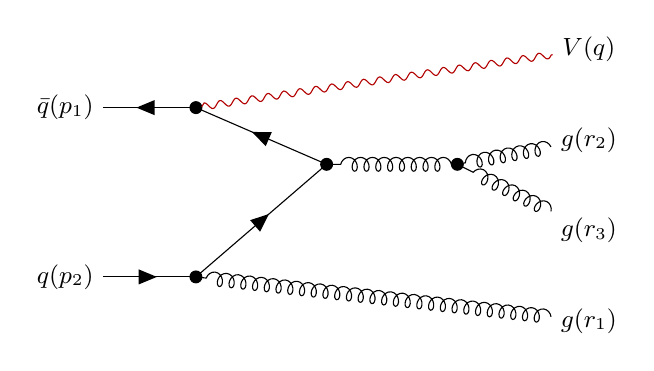
\begin{tikzpicture}[baseline=(current bounding box.center)]
\begin{feynman}
\vertex (e1) at (0.43,3.00) {\small $\bar q(p_1)$};
\vertex (e3) at (0.43,0.85) {\small $q(p_2)$};
\vertex (e5) at (7.08,3.74) {\small $V(q)$};
\vertex (e7) at (7.08,0.29) {\small $g(r_1)$};
\vertex (e9) at (7.08,2.59) {\small $g(r_2)$};
\vertex (e11) at (7.08,1.44) {\small $g(r_3)$};
\vertex[dot] (v0) at (2.09,3.00) {};
\vertex[dot] (v1) at (2.09,0.85) {};
\vertex[dot] (v2) at (5.41,2.28) {};
\vertex[dot] (v3) at (3.75,2.28) {};
\diagram* {
(v0) -- [fermion] (e1),
(e3) -- [fermion] (v1),
(e5) -- [boson, red!70!black] (v0),
(e7) -- [gluon] (v1),
(e9) -- [gluon] (v2),
(e11) -- [gluon] (v2),
(v3) -- [fermion] (v0),
(v1) -- [fermion] (v3),
(v2) -- [gluon] (v3),
};
\end{feynman}
\end{tikzpicture}}\\[2mm]\textbf{Vqbqggg}: $\bar q q \to V\, g g g$\\ {\footnotesize diagram 3 of 50, p1$\leftrightarrow$p2 partner Vqqbggg}\end{minipage}\hfill%


\section*{\texttt{physical\_qqbQ2Q2bg}}
\begin{minipage}[t]{0.48\textwidth}\centering\resizebox{0.95\linewidth}{!}{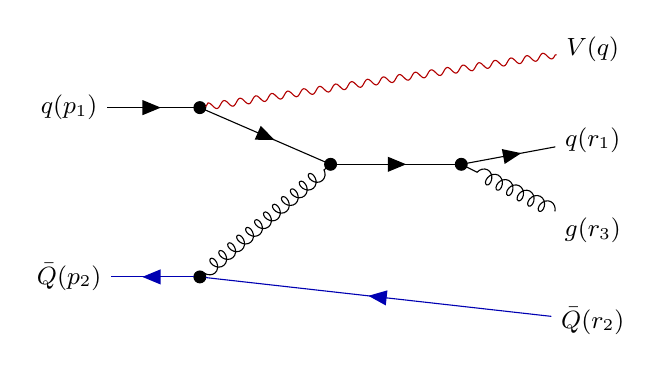
\begin{tikzpicture}[baseline=(current bounding box.center)]
\begin{feynman}
\vertex (e1) at (0.43,3.00) {\small $q(p_1)$};
\vertex (e3) at (0.43,0.85) {\small $\bar Q(p_2)$};
\vertex (e5) at (7.08,3.74) {\small $V(q)$};
\vertex (e7) at (7.08,2.59) {\small $q(r_1)$};
\vertex (e9) at (7.08,0.29) {\small $\bar Q(r_2)$};
\vertex (e11) at (7.08,1.44) {\small $g(r_3)$};
\vertex[dot] (v0) at (2.09,3.00) {};
\vertex[dot] (v1) at (2.09,0.85) {};
\vertex[dot] (v2) at (5.41,2.28) {};
\vertex[dot] (v3) at (3.75,2.28) {};
\diagram* {
(e1) -- [fermion] (v0),
(v1) -- [fermion, blue!70!black] (e3),
(e5) -- [boson, red!70!black] (v0),
(v2) -- [fermion] (e7),
(e9) -- [fermion, blue!70!black] (v1),
(e11) -- [gluon] (v2),
(v0) -- [fermion] (v3),
(v1) -- [gluon] (v3),
(v3) -- [fermion] (v2),
};
\end{feynman}
\end{tikzpicture}}\\[2mm]\textbf{VqQ2bqQ2bg}: $q \bar Q \to V\, q \bar Q g$\\ {\footnotesize diagram 1 of 24, p1$\leftrightarrow$p2 partner VQ2bqqQ2bg}\end{minipage}\hfill%
\begin{minipage}[t]{0.48\textwidth}\centering\resizebox{0.95\linewidth}{!}{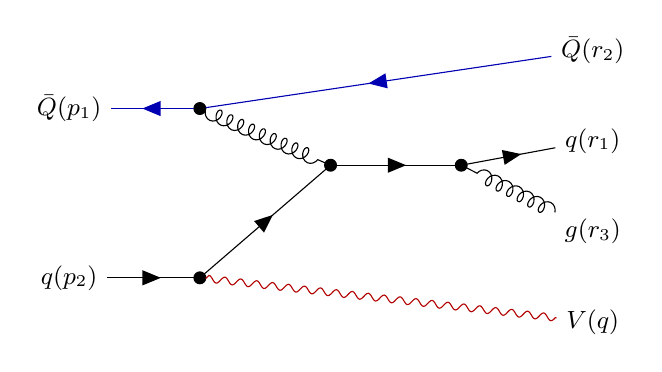
\begin{tikzpicture}[baseline=(current bounding box.center)]
\begin{feynman}
\vertex (e1) at (0.43,3.00) {\small $\bar Q(p_1)$};
\vertex (e3) at (0.43,0.85) {\small $q(p_2)$};
\vertex (e5) at (7.08,0.29) {\small $V(q)$};
\vertex (e7) at (7.08,2.59) {\small $q(r_1)$};
\vertex (e9) at (7.08,3.74) {\small $\bar Q(r_2)$};
\vertex (e11) at (7.08,1.44) {\small $g(r_3)$};
\vertex[dot] (v0) at (2.09,3.00) {};
\vertex[dot] (v1) at (2.09,0.85) {};
\vertex[dot] (v2) at (5.41,2.28) {};
\vertex[dot] (v3) at (3.75,2.28) {};
\diagram* {
(v0) -- [fermion, blue!70!black] (e1),
(e3) -- [fermion] (v1),
(e5) -- [boson, red!70!black] (v1),
(v2) -- [fermion] (e7),
(e9) -- [fermion, blue!70!black] (v0),
(e11) -- [gluon] (v2),
(v0) -- [gluon] (v3),
(v1) -- [fermion] (v3),
(v3) -- [fermion] (v2),
};
\end{feynman}
\end{tikzpicture}}\\[2mm]\textbf{VQ2bqqQ2bg}: $\bar Q q \to V\, q \bar Q g$\\ {\footnotesize diagram 2 of 24, p1$\leftrightarrow$p2 partner VqQ2bqQ2bg}\end{minipage}\hfill

\bigskip

\begin{minipage}[t]{0.48\textwidth}\centering\resizebox{0.95\linewidth}{!}{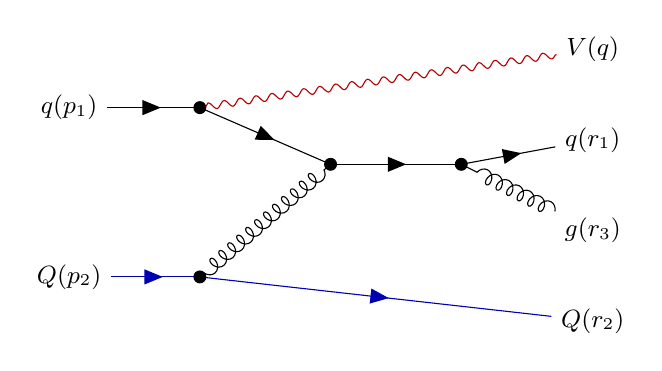
\begin{tikzpicture}[baseline=(current bounding box.center)]
\begin{feynman}
\vertex (e1) at (0.43,3.00) {\small $q(p_1)$};
\vertex (e3) at (0.43,0.85) {\small $Q(p_2)$};
\vertex (e5) at (7.08,3.74) {\small $V(q)$};
\vertex (e7) at (7.08,2.59) {\small $q(r_1)$};
\vertex (e9) at (7.08,0.29) {\small $Q(r_2)$};
\vertex (e11) at (7.08,1.44) {\small $g(r_3)$};
\vertex[dot] (v0) at (2.09,3.00) {};
\vertex[dot] (v1) at (2.09,0.85) {};
\vertex[dot] (v2) at (5.41,2.28) {};
\vertex[dot] (v3) at (3.75,2.28) {};
\diagram* {
(e1) -- [fermion] (v0),
(e3) -- [fermion, blue!70!black] (v1),
(e5) -- [boson, red!70!black] (v0),
(v2) -- [fermion] (e7),
(v1) -- [fermion, blue!70!black] (e9),
(e11) -- [gluon] (v2),
(v0) -- [fermion] (v3),
(v1) -- [gluon] (v3),
(v3) -- [fermion] (v2),
};
\end{feynman}
\end{tikzpicture}}\\[2mm]\textbf{VqQ2qQ2g}: $q Q \to V\, q Q g$\\ {\footnotesize diagram 1 of 24, p1$\leftrightarrow$p2 partner VQ2qqQ2g}\end{minipage}\hfill%
\begin{minipage}[t]{0.48\textwidth}\centering\resizebox{0.95\linewidth}{!}{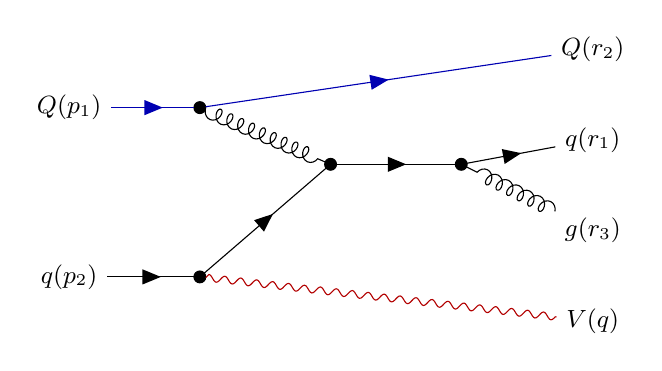
\begin{tikzpicture}[baseline=(current bounding box.center)]
\begin{feynman}
\vertex (e1) at (0.43,3.00) {\small $Q(p_1)$};
\vertex (e3) at (0.43,0.85) {\small $q(p_2)$};
\vertex (e5) at (7.08,0.29) {\small $V(q)$};
\vertex (e7) at (7.08,2.59) {\small $q(r_1)$};
\vertex (e9) at (7.08,3.74) {\small $Q(r_2)$};
\vertex (e11) at (7.08,1.44) {\small $g(r_3)$};
\vertex[dot] (v0) at (2.09,3.00) {};
\vertex[dot] (v1) at (2.09,0.85) {};
\vertex[dot] (v2) at (5.41,2.28) {};
\vertex[dot] (v3) at (3.75,2.28) {};
\diagram* {
(e1) -- [fermion, blue!70!black] (v0),
(e3) -- [fermion] (v1),
(e5) -- [boson, red!70!black] (v1),
(v2) -- [fermion] (e7),
(v0) -- [fermion, blue!70!black] (e9),
(e11) -- [gluon] (v2),
(v0) -- [gluon] (v3),
(v1) -- [fermion] (v3),
(v3) -- [fermion] (v2),
};
\end{feynman}
\end{tikzpicture}}\\[2mm]\textbf{VQ2qqQ2g}: $Q q \to V\, q Q g$\\ {\footnotesize diagram 2 of 24, p1$\leftrightarrow$p2 partner VqQ2qQ2g}\end{minipage}\hfill

\bigskip

\begin{minipage}[t]{0.48\textwidth}\centering\resizebox{0.95\linewidth}{!}{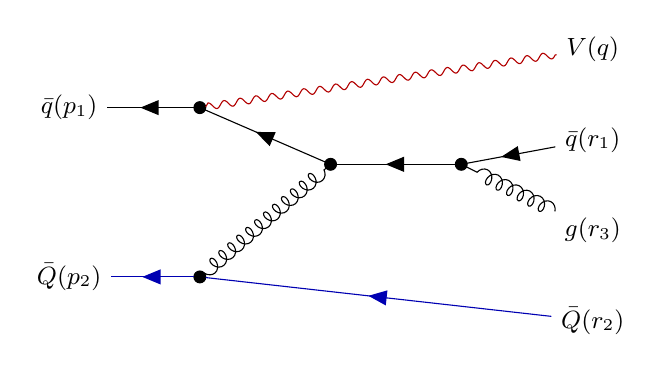
\begin{tikzpicture}[baseline=(current bounding box.center)]
\begin{feynman}
\vertex (e1) at (0.43,3.00) {\small $\bar q(p_1)$};
\vertex (e3) at (0.43,0.85) {\small $\bar Q(p_2)$};
\vertex (e5) at (7.08,3.74) {\small $V(q)$};
\vertex (e7) at (7.08,2.59) {\small $\bar q(r_1)$};
\vertex (e9) at (7.08,0.29) {\small $\bar Q(r_2)$};
\vertex (e11) at (7.08,1.44) {\small $g(r_3)$};
\vertex[dot] (v0) at (2.09,3.00) {};
\vertex[dot] (v1) at (2.09,0.85) {};
\vertex[dot] (v2) at (5.41,2.28) {};
\vertex[dot] (v3) at (3.75,2.28) {};
\diagram* {
(v0) -- [fermion] (e1),
(v1) -- [fermion, blue!70!black] (e3),
(e5) -- [boson, red!70!black] (v0),
(e7) -- [fermion] (v2),
(e9) -- [fermion, blue!70!black] (v1),
(e11) -- [gluon] (v2),
(v3) -- [fermion] (v0),
(v1) -- [gluon] (v3),
(v2) -- [fermion] (v3),
};
\end{feynman}
\end{tikzpicture}}\\[2mm]\textbf{VqbQ2bqbQ2bg}: $\bar q \bar Q \to V\, \bar q \bar Q g$\\ {\footnotesize diagram 1 of 24, p1$\leftrightarrow$p2 partner VQ2bqbqbQ2bg}\end{minipage}\hfill%
\begin{minipage}[t]{0.48\textwidth}\centering\resizebox{0.95\linewidth}{!}{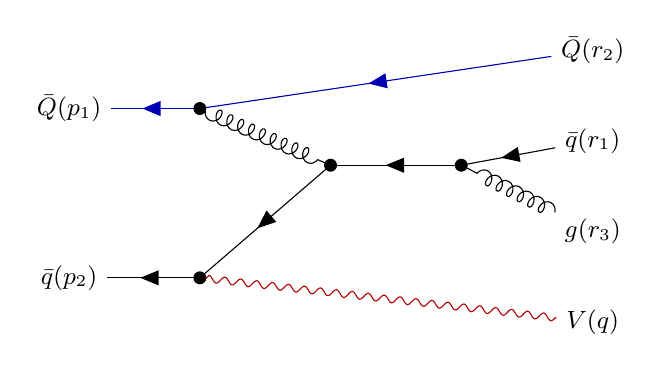
\begin{tikzpicture}[baseline=(current bounding box.center)]
\begin{feynman}
\vertex (e1) at (0.43,3.00) {\small $\bar Q(p_1)$};
\vertex (e3) at (0.43,0.85) {\small $\bar q(p_2)$};
\vertex (e5) at (7.08,0.29) {\small $V(q)$};
\vertex (e7) at (7.08,2.59) {\small $\bar q(r_1)$};
\vertex (e9) at (7.08,3.74) {\small $\bar Q(r_2)$};
\vertex (e11) at (7.08,1.44) {\small $g(r_3)$};
\vertex[dot] (v0) at (2.09,3.00) {};
\vertex[dot] (v1) at (2.09,0.85) {};
\vertex[dot] (v2) at (5.41,2.28) {};
\vertex[dot] (v3) at (3.75,2.28) {};
\diagram* {
(v0) -- [fermion, blue!70!black] (e1),
(v1) -- [fermion] (e3),
(e5) -- [boson, red!70!black] (v1),
(e7) -- [fermion] (v2),
(e9) -- [fermion, blue!70!black] (v0),
(e11) -- [gluon] (v2),
(v0) -- [gluon] (v3),
(v3) -- [fermion] (v1),
(v2) -- [fermion] (v3),
};
\end{feynman}
\end{tikzpicture}}\\[2mm]\textbf{VQ2bqbqbQ2bg}: $\bar Q \bar q \to V\, \bar q \bar Q g$\\ {\footnotesize diagram 2 of 24, p1$\leftrightarrow$p2 partner VqbQ2bqbQ2bg}\end{minipage}\hfill

\bigskip

\begin{minipage}[t]{0.48\textwidth}\centering\resizebox{0.95\linewidth}{!}{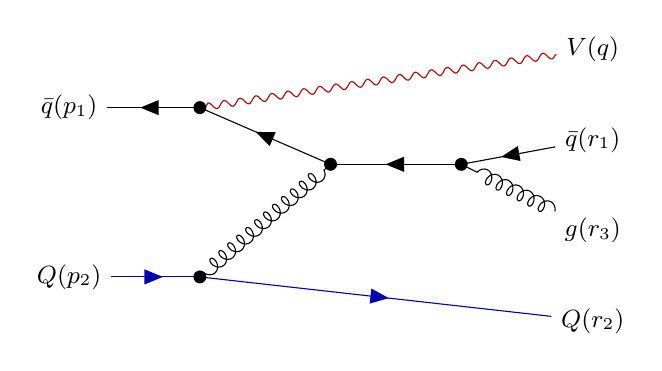
\begin{tikzpicture}[baseline=(current bounding box.center)]
\begin{feynman}
\vertex (e1) at (0.43,3.00) {\small $\bar q(p_1)$};
\vertex (e3) at (0.43,0.85) {\small $Q(p_2)$};
\vertex (e5) at (7.08,3.74) {\small $V(q)$};
\vertex (e7) at (7.08,2.59) {\small $\bar q(r_1)$};
\vertex (e9) at (7.08,0.29) {\small $Q(r_2)$};
\vertex (e11) at (7.08,1.44) {\small $g(r_3)$};
\vertex[dot] (v0) at (2.09,3.00) {};
\vertex[dot] (v1) at (2.09,0.85) {};
\vertex[dot] (v2) at (5.41,2.28) {};
\vertex[dot] (v3) at (3.75,2.28) {};
\diagram* {
(v0) -- [fermion] (e1),
(e3) -- [fermion, blue!70!black] (v1),
(e5) -- [boson, red!70!black] (v0),
(e7) -- [fermion] (v2),
(v1) -- [fermion, blue!70!black] (e9),
(e11) -- [gluon] (v2),
(v3) -- [fermion] (v0),
(v1) -- [gluon] (v3),
(v2) -- [fermion] (v3),
};
\end{feynman}
\end{tikzpicture}}\\[2mm]\textbf{VqbQ2qbQ2g}: $\bar q Q \to V\, \bar q Q g$\\ {\footnotesize diagram 1 of 24, p1$\leftrightarrow$p2 partner VQ2qbqbQ2g}\end{minipage}\hfill%
\begin{minipage}[t]{0.48\textwidth}\centering\resizebox{0.95\linewidth}{!}{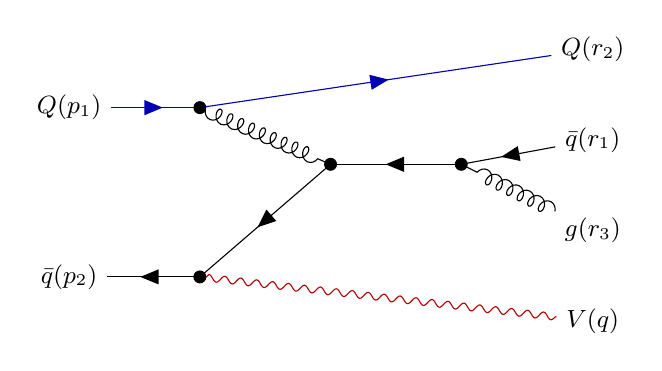
\begin{tikzpicture}[baseline=(current bounding box.center)]
\begin{feynman}
\vertex (e1) at (0.43,3.00) {\small $Q(p_1)$};
\vertex (e3) at (0.43,0.85) {\small $\bar q(p_2)$};
\vertex (e5) at (7.08,0.29) {\small $V(q)$};
\vertex (e7) at (7.08,2.59) {\small $\bar q(r_1)$};
\vertex (e9) at (7.08,3.74) {\small $Q(r_2)$};
\vertex (e11) at (7.08,1.44) {\small $g(r_3)$};
\vertex[dot] (v0) at (2.09,3.00) {};
\vertex[dot] (v1) at (2.09,0.85) {};
\vertex[dot] (v2) at (5.41,2.28) {};
\vertex[dot] (v3) at (3.75,2.28) {};
\diagram* {
(e1) -- [fermion, blue!70!black] (v0),
(v1) -- [fermion] (e3),
(e5) -- [boson, red!70!black] (v1),
(e7) -- [fermion] (v2),
(v0) -- [fermion, blue!70!black] (e9),
(e11) -- [gluon] (v2),
(v0) -- [gluon] (v3),
(v3) -- [fermion] (v1),
(v2) -- [fermion] (v3),
};
\end{feynman}
\end{tikzpicture}}\\[2mm]\textbf{VQ2qbqbQ2g}: $Q \bar q \to V\, \bar q Q g$\\ {\footnotesize diagram 2 of 24, p1$\leftrightarrow$p2 partner VqbQ2qbQ2g}\end{minipage}\hfill

\bigskip

\begin{minipage}[t]{0.48\textwidth}\centering\resizebox{0.95\linewidth}{!}{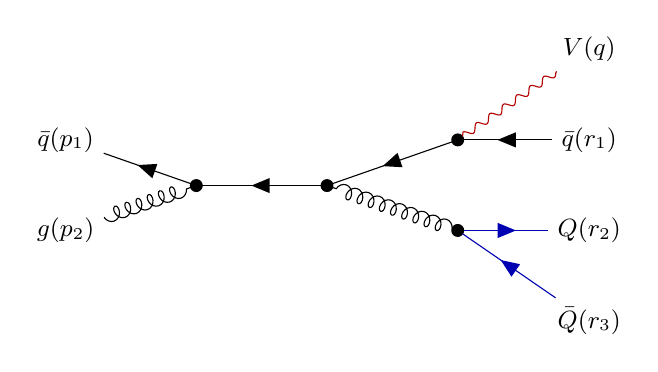
\begin{tikzpicture}[baseline=(current bounding box.center)]
\begin{feynman}
\vertex (e1) at (0.43,2.59) {\small $\bar q(p_1)$};
\vertex (e3) at (0.43,1.44) {\small $g(p_2)$};
\vertex (e5) at (7.08,3.74) {\small $V(q)$};
\vertex (e7) at (7.08,2.59) {\small $\bar q(r_1)$};
\vertex (e9) at (7.08,1.44) {\small $Q(r_2)$};
\vertex (e11) at (7.08,0.29) {\small $\bar Q(r_3)$};
\vertex[dot] (v0) at (2.09,2.01) {};
\vertex[dot] (v1) at (5.41,2.59) {};
\vertex[dot] (v2) at (5.41,1.44) {};
\vertex[dot] (v3) at (3.75,2.01) {};
\diagram* {
(v0) -- [fermion] (e1),
(e3) -- [gluon] (v0),
(e5) -- [boson, red!70!black] (v1),
(e7) -- [fermion] (v1),
(v2) -- [fermion, blue!70!black] (e9),
(e11) -- [fermion, blue!70!black] (v2),
(v3) -- [fermion] (v0),
(v1) -- [fermion] (v3),
(v2) -- [gluon] (v3),
};
\end{feynman}
\end{tikzpicture}}\\[2mm]\textbf{VqbgqbQ2Q2b}: $\bar q g \to V\, \bar q Q \bar Q$\\ {\footnotesize diagram 1 of 24, p1$\leftrightarrow$p2 partner VgqbqbQ2Q2b}\end{minipage}\hfill%
\begin{minipage}[t]{0.48\textwidth}\centering\resizebox{0.95\linewidth}{!}{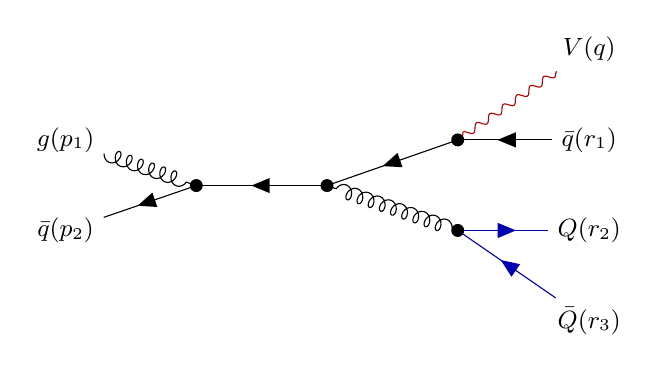
\begin{tikzpicture}[baseline=(current bounding box.center)]
\begin{feynman}
\vertex (e1) at (0.43,2.59) {\small $g(p_1)$};
\vertex (e3) at (0.43,1.44) {\small $\bar q(p_2)$};
\vertex (e5) at (7.08,3.74) {\small $V(q)$};
\vertex (e7) at (7.08,2.59) {\small $\bar q(r_1)$};
\vertex (e9) at (7.08,1.44) {\small $Q(r_2)$};
\vertex (e11) at (7.08,0.29) {\small $\bar Q(r_3)$};
\vertex[dot] (v0) at (2.09,2.01) {};
\vertex[dot] (v1) at (5.41,2.59) {};
\vertex[dot] (v2) at (5.41,1.44) {};
\vertex[dot] (v3) at (3.75,2.01) {};
\diagram* {
(e1) -- [gluon] (v0),
(v0) -- [fermion] (e3),
(e5) -- [boson, red!70!black] (v1),
(e7) -- [fermion] (v1),
(v2) -- [fermion, blue!70!black] (e9),
(e11) -- [fermion, blue!70!black] (v2),
(v3) -- [fermion] (v0),
(v1) -- [fermion] (v3),
(v2) -- [gluon] (v3),
};
\end{feynman}
\end{tikzpicture}}\\[2mm]\textbf{VgqbqbQ2Q2b}: $g \bar q \to V\, \bar q Q \bar Q$\\ {\footnotesize diagram 1 of 24, p1$\leftrightarrow$p2 partner VqbgqbQ2Q2b}\end{minipage}\hfill

\bigskip

\begin{minipage}[t]{0.48\textwidth}\centering\resizebox{0.95\linewidth}{!}{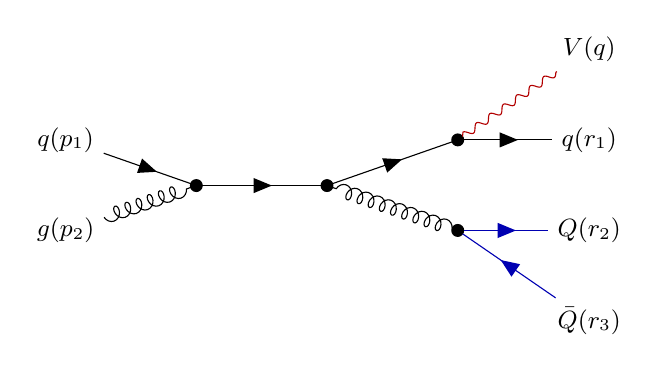
\begin{tikzpicture}[baseline=(current bounding box.center)]
\begin{feynman}
\vertex (e1) at (0.43,2.59) {\small $q(p_1)$};
\vertex (e3) at (0.43,1.44) {\small $g(p_2)$};
\vertex (e5) at (7.08,3.74) {\small $V(q)$};
\vertex (e7) at (7.08,2.59) {\small $q(r_1)$};
\vertex (e9) at (7.08,1.44) {\small $Q(r_2)$};
\vertex (e11) at (7.08,0.29) {\small $\bar Q(r_3)$};
\vertex[dot] (v0) at (2.09,2.01) {};
\vertex[dot] (v1) at (5.41,2.59) {};
\vertex[dot] (v2) at (5.41,1.44) {};
\vertex[dot] (v3) at (3.75,2.01) {};
\diagram* {
(e1) -- [fermion] (v0),
(e3) -- [gluon] (v0),
(e5) -- [boson, red!70!black] (v1),
(v1) -- [fermion] (e7),
(v2) -- [fermion, blue!70!black] (e9),
(e11) -- [fermion, blue!70!black] (v2),
(v0) -- [fermion] (v3),
(v3) -- [fermion] (v1),
(v2) -- [gluon] (v3),
};
\end{feynman}
\end{tikzpicture}}\\[2mm]\textbf{VqgqQ2Q2b}: $q g \to V\, q Q \bar Q$\\ {\footnotesize diagram 1 of 24, p1$\leftrightarrow$p2 partner VgqqQ2Q2b}\end{minipage}\hfill%
\begin{minipage}[t]{0.48\textwidth}\centering\resizebox{0.95\linewidth}{!}{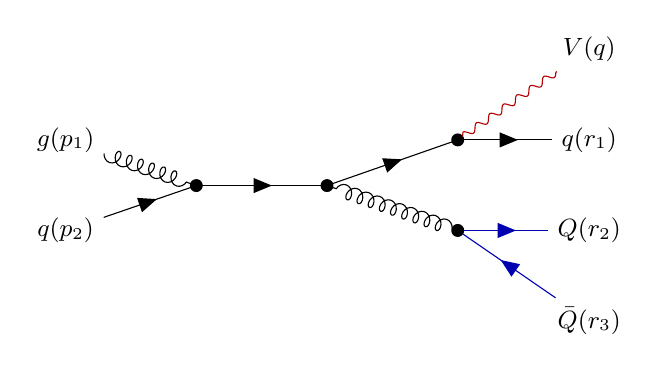
\begin{tikzpicture}[baseline=(current bounding box.center)]
\begin{feynman}
\vertex (e1) at (0.43,2.59) {\small $g(p_1)$};
\vertex (e3) at (0.43,1.44) {\small $q(p_2)$};
\vertex (e5) at (7.08,3.74) {\small $V(q)$};
\vertex (e7) at (7.08,2.59) {\small $q(r_1)$};
\vertex (e9) at (7.08,1.44) {\small $Q(r_2)$};
\vertex (e11) at (7.08,0.29) {\small $\bar Q(r_3)$};
\vertex[dot] (v0) at (2.09,2.01) {};
\vertex[dot] (v1) at (5.41,2.59) {};
\vertex[dot] (v2) at (5.41,1.44) {};
\vertex[dot] (v3) at (3.75,2.01) {};
\diagram* {
(e1) -- [gluon] (v0),
(e3) -- [fermion] (v0),
(e5) -- [boson, red!70!black] (v1),
(v1) -- [fermion] (e7),
(v2) -- [fermion, blue!70!black] (e9),
(e11) -- [fermion, blue!70!black] (v2),
(v0) -- [fermion] (v3),
(v3) -- [fermion] (v1),
(v2) -- [gluon] (v3),
};
\end{feynman}
\end{tikzpicture}}\\[2mm]\textbf{VgqqQ2Q2b}: $g q \to V\, q Q \bar Q$\\ {\footnotesize diagram 1 of 24, p1$\leftrightarrow$p2 partner VqgqQ2Q2b}\end{minipage}\hfill

\bigskip

\begin{minipage}[t]{0.48\textwidth}\centering\resizebox{0.95\linewidth}{!}{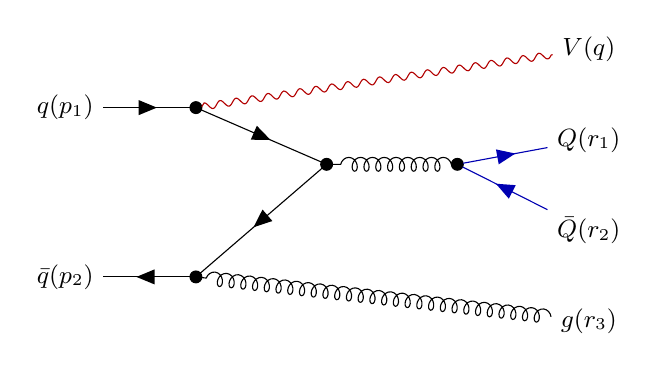
\begin{tikzpicture}[baseline=(current bounding box.center)]
\begin{feynman}
\vertex (e1) at (0.43,3.00) {\small $q(p_1)$};
\vertex (e3) at (0.43,0.85) {\small $\bar q(p_2)$};
\vertex (e5) at (7.08,3.74) {\small $V(q)$};
\vertex (e7) at (7.08,2.59) {\small $Q(r_1)$};
\vertex (e9) at (7.08,1.44) {\small $\bar Q(r_2)$};
\vertex (e11) at (7.08,0.29) {\small $g(r_3)$};
\vertex[dot] (v0) at (2.09,3.00) {};
\vertex[dot] (v1) at (2.09,0.85) {};
\vertex[dot] (v2) at (5.41,2.28) {};
\vertex[dot] (v3) at (3.75,2.28) {};
\diagram* {
(e1) -- [fermion] (v0),
(v1) -- [fermion] (e3),
(e5) -- [boson, red!70!black] (v0),
(v2) -- [fermion, blue!70!black] (e7),
(e9) -- [fermion, blue!70!black] (v2),
(e11) -- [gluon] (v1),
(v0) -- [fermion] (v3),
(v3) -- [fermion] (v1),
(v2) -- [gluon] (v3),
};
\end{feynman}
\end{tikzpicture}}\\[2mm]\textbf{VqqbQ2Q2bg}: $q \bar q \to V\, Q \bar Q g$\\ {\footnotesize diagram 3 of 24, p1$\leftrightarrow$p2 partner VqbqQ2Q2bg}\end{minipage}\hfill%
\begin{minipage}[t]{0.48\textwidth}\centering\resizebox{0.95\linewidth}{!}{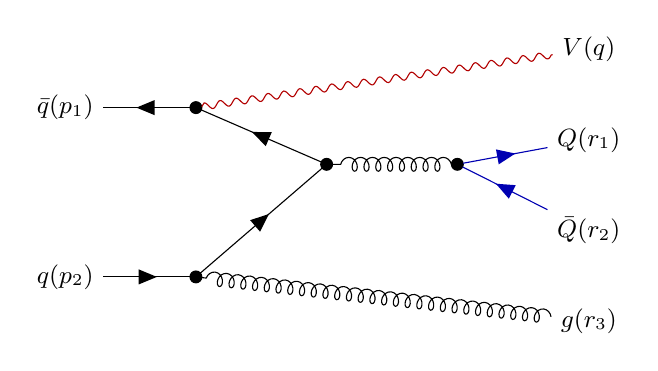
\begin{tikzpicture}[baseline=(current bounding box.center)]
\begin{feynman}
\vertex (e1) at (0.43,3.00) {\small $\bar q(p_1)$};
\vertex (e3) at (0.43,0.85) {\small $q(p_2)$};
\vertex (e5) at (7.08,3.74) {\small $V(q)$};
\vertex (e7) at (7.08,2.59) {\small $Q(r_1)$};
\vertex (e9) at (7.08,1.44) {\small $\bar Q(r_2)$};
\vertex (e11) at (7.08,0.29) {\small $g(r_3)$};
\vertex[dot] (v0) at (2.09,3.00) {};
\vertex[dot] (v1) at (2.09,0.85) {};
\vertex[dot] (v2) at (5.41,2.28) {};
\vertex[dot] (v3) at (3.75,2.28) {};
\diagram* {
(v0) -- [fermion] (e1),
(e3) -- [fermion] (v1),
(e5) -- [boson, red!70!black] (v0),
(v2) -- [fermion, blue!70!black] (e7),
(e9) -- [fermion, blue!70!black] (v2),
(e11) -- [gluon] (v1),
(v3) -- [fermion] (v0),
(v1) -- [fermion] (v3),
(v2) -- [gluon] (v3),
};
\end{feynman}
\end{tikzpicture}}\\[2mm]\textbf{VqbqQ2Q2bg}: $\bar q q \to V\, Q \bar Q g$\\ {\footnotesize diagram 3 of 24, p1$\leftrightarrow$p2 partner VqqbQ2Q2bg}\end{minipage}\hfill

\bigskip

\section*{\texttt{physical\_qqbqqbg}}
\begin{minipage}[t]{0.48\textwidth}\centering\resizebox{0.95\linewidth}{!}{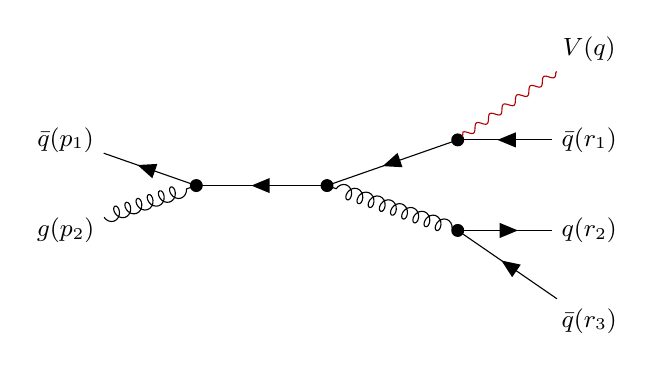
\begin{tikzpicture}[baseline=(current bounding box.center)]
\begin{feynman}
\vertex (e1) at (0.43,2.59) {\small $\bar q(p_1)$};
\vertex (e3) at (0.43,1.44) {\small $g(p_2)$};
\vertex (e5) at (7.08,3.74) {\small $V(q)$};
\vertex (e7) at (7.08,2.59) {\small $\bar q(r_1)$};
\vertex (e9) at (7.08,1.44) {\small $q(r_2)$};
\vertex (e11) at (7.08,0.29) {\small $\bar q(r_3)$};
\vertex[dot] (v0) at (2.09,2.01) {};
\vertex[dot] (v1) at (5.41,2.59) {};
\vertex[dot] (v2) at (5.41,1.44) {};
\vertex[dot] (v3) at (3.75,2.01) {};
\diagram* {
(v0) -- [fermion] (e1),
(e3) -- [gluon] (v0),
(e5) -- [boson, red!70!black] (v1),
(e7) -- [fermion] (v1),
(v2) -- [fermion] (e9),
(e11) -- [fermion] (v2),
(v3) -- [fermion] (v0),
(v1) -- [fermion] (v3),
(v2) -- [gluon] (v3),
};
\end{feynman}
\end{tikzpicture}}\\[2mm]\textbf{Vqbgqbqqb}: $\bar q g \to V\, \bar q q \bar q$\\ {\footnotesize diagram 1 of 48, p1$\leftrightarrow$p2 partner Vgqbqbqqb}\end{minipage}\hfill%
\begin{minipage}[t]{0.48\textwidth}\centering\resizebox{0.95\linewidth}{!}{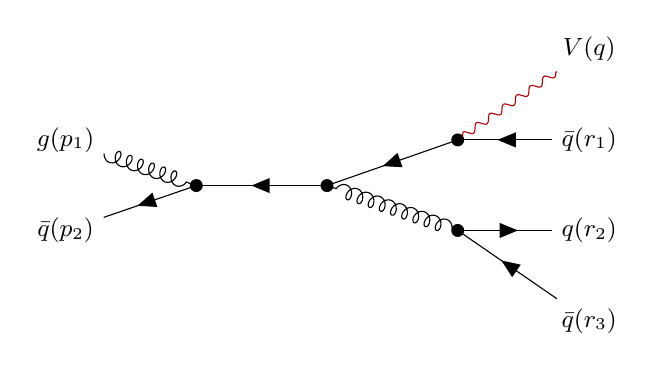
\begin{tikzpicture}[baseline=(current bounding box.center)]
\begin{feynman}
\vertex (e1) at (0.43,2.59) {\small $g(p_1)$};
\vertex (e3) at (0.43,1.44) {\small $\bar q(p_2)$};
\vertex (e5) at (7.08,3.74) {\small $V(q)$};
\vertex (e7) at (7.08,2.59) {\small $\bar q(r_1)$};
\vertex (e9) at (7.08,1.44) {\small $q(r_2)$};
\vertex (e11) at (7.08,0.29) {\small $\bar q(r_3)$};
\vertex[dot] (v0) at (2.09,2.01) {};
\vertex[dot] (v1) at (5.41,2.59) {};
\vertex[dot] (v2) at (5.41,1.44) {};
\vertex[dot] (v3) at (3.75,2.01) {};
\diagram* {
(e1) -- [gluon] (v0),
(v0) -- [fermion] (e3),
(e5) -- [boson, red!70!black] (v1),
(e7) -- [fermion] (v1),
(v2) -- [fermion] (e9),
(e11) -- [fermion] (v2),
(v3) -- [fermion] (v0),
(v1) -- [fermion] (v3),
(v2) -- [gluon] (v3),
};
\end{feynman}
\end{tikzpicture}}\\[2mm]\textbf{Vgqbqbqqb}: $g \bar q \to V\, \bar q q \bar q$\\ {\footnotesize diagram 1 of 48, p1$\leftrightarrow$p2 partner Vqbgqbqqb}\end{minipage}\hfill

\bigskip

\begin{minipage}[t]{0.48\textwidth}\centering\resizebox{0.95\linewidth}{!}{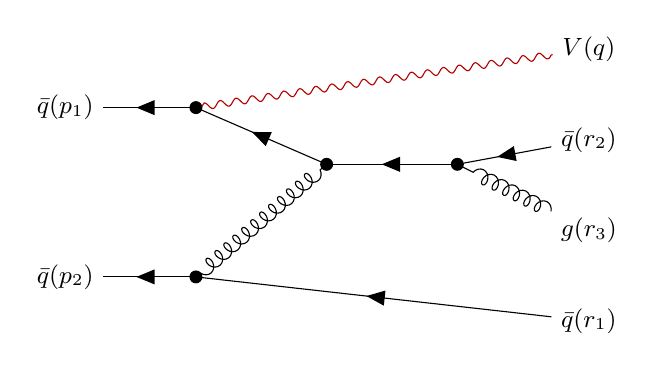
\begin{tikzpicture}[baseline=(current bounding box.center)]
\begin{feynman}
\vertex (e1) at (0.43,3.00) {\small $\bar q(p_1)$};
\vertex (e3) at (0.43,0.85) {\small $\bar q(p_2)$};
\vertex (e5) at (7.08,3.74) {\small $V(q)$};
\vertex (e7) at (7.08,0.29) {\small $\bar q(r_1)$};
\vertex (e9) at (7.08,2.59) {\small $\bar q(r_2)$};
\vertex (e11) at (7.08,1.44) {\small $g(r_3)$};
\vertex[dot] (v0) at (2.09,3.00) {};
\vertex[dot] (v1) at (2.09,0.85) {};
\vertex[dot] (v2) at (5.41,2.28) {};
\vertex[dot] (v3) at (3.75,2.28) {};
\diagram* {
(v0) -- [fermion] (e1),
(v1) -- [fermion] (e3),
(e5) -- [boson, red!70!black] (v0),
(e7) -- [fermion] (v1),
(e9) -- [fermion] (v2),
(e11) -- [gluon] (v2),
(v3) -- [fermion] (v0),
(v1) -- [gluon] (v3),
(v2) -- [fermion] (v3),
};
\end{feynman}
\end{tikzpicture}}\\[2mm]\textbf{Vqbqbqbqbg}: $\bar q \bar q \to V\, \bar q \bar q g$\\ {\footnotesize diagram 1 of 48, p1$\leftrightarrow$p2 symmetric}\end{minipage}\hfill%
\begin{minipage}[t]{0.48\textwidth}\centering\resizebox{0.95\linewidth}{!}{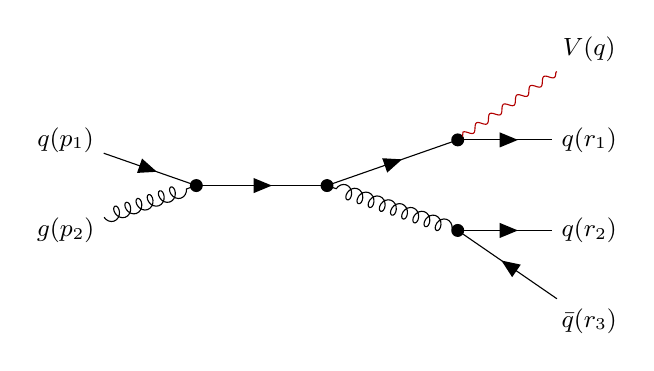
\begin{tikzpicture}[baseline=(current bounding box.center)]
\begin{feynman}
\vertex (e1) at (0.43,2.59) {\small $q(p_1)$};
\vertex (e3) at (0.43,1.44) {\small $g(p_2)$};
\vertex (e5) at (7.08,3.74) {\small $V(q)$};
\vertex (e7) at (7.08,2.59) {\small $q(r_1)$};
\vertex (e9) at (7.08,1.44) {\small $q(r_2)$};
\vertex (e11) at (7.08,0.29) {\small $\bar q(r_3)$};
\vertex[dot] (v0) at (2.09,2.01) {};
\vertex[dot] (v1) at (5.41,2.59) {};
\vertex[dot] (v2) at (5.41,1.44) {};
\vertex[dot] (v3) at (3.75,2.01) {};
\diagram* {
(e1) -- [fermion] (v0),
(e3) -- [gluon] (v0),
(e5) -- [boson, red!70!black] (v1),
(v1) -- [fermion] (e7),
(v2) -- [fermion] (e9),
(e11) -- [fermion] (v2),
(v0) -- [fermion] (v3),
(v3) -- [fermion] (v1),
(v2) -- [gluon] (v3),
};
\end{feynman}
\end{tikzpicture}}\\[2mm]\textbf{Vqgqqqb}: $q g \to V\, q q \bar q$\\ {\footnotesize diagram 1 of 48, p1$\leftrightarrow$p2 partner Vgqqqqb}\end{minipage}\hfill

\bigskip

\begin{minipage}[t]{0.48\textwidth}\centering\resizebox{0.95\linewidth}{!}{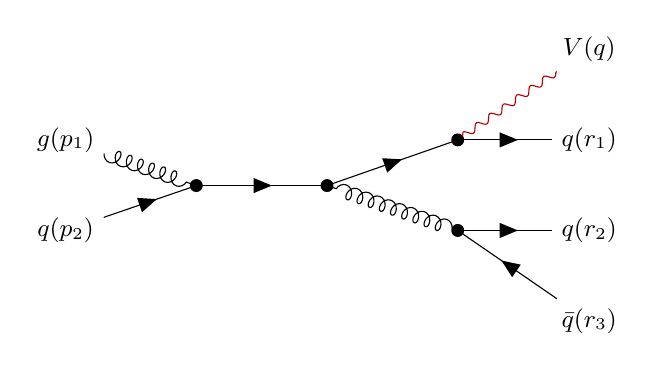
\begin{tikzpicture}[baseline=(current bounding box.center)]
\begin{feynman}
\vertex (e1) at (0.43,2.59) {\small $g(p_1)$};
\vertex (e3) at (0.43,1.44) {\small $q(p_2)$};
\vertex (e5) at (7.08,3.74) {\small $V(q)$};
\vertex (e7) at (7.08,2.59) {\small $q(r_1)$};
\vertex (e9) at (7.08,1.44) {\small $q(r_2)$};
\vertex (e11) at (7.08,0.29) {\small $\bar q(r_3)$};
\vertex[dot] (v0) at (2.09,2.01) {};
\vertex[dot] (v1) at (5.41,2.59) {};
\vertex[dot] (v2) at (5.41,1.44) {};
\vertex[dot] (v3) at (3.75,2.01) {};
\diagram* {
(e1) -- [gluon] (v0),
(e3) -- [fermion] (v0),
(e5) -- [boson, red!70!black] (v1),
(v1) -- [fermion] (e7),
(v2) -- [fermion] (e9),
(e11) -- [fermion] (v2),
(v0) -- [fermion] (v3),
(v3) -- [fermion] (v1),
(v2) -- [gluon] (v3),
};
\end{feynman}
\end{tikzpicture}}\\[2mm]\textbf{Vgqqqqb}: $g q \to V\, q q \bar q$\\ {\footnotesize diagram 1 of 48, p1$\leftrightarrow$p2 partner Vqgqqqb}\end{minipage}\hfill%
\begin{minipage}[t]{0.48\textwidth}\centering\resizebox{0.95\linewidth}{!}{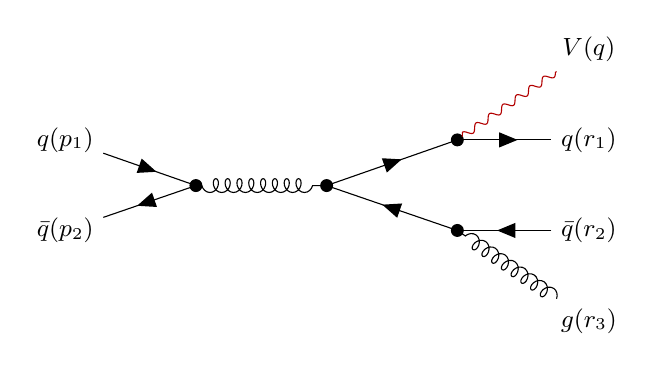
\begin{tikzpicture}[baseline=(current bounding box.center)]
\begin{feynman}
\vertex (e1) at (0.43,2.59) {\small $q(p_1)$};
\vertex (e3) at (0.43,1.44) {\small $\bar q(p_2)$};
\vertex (e5) at (7.08,3.74) {\small $V(q)$};
\vertex (e7) at (7.08,2.59) {\small $q(r_1)$};
\vertex (e9) at (7.08,1.44) {\small $\bar q(r_2)$};
\vertex (e11) at (7.08,0.29) {\small $g(r_3)$};
\vertex[dot] (v0) at (2.09,2.01) {};
\vertex[dot] (v1) at (5.41,2.59) {};
\vertex[dot] (v2) at (5.41,1.44) {};
\vertex[dot] (v3) at (3.75,2.01) {};
\diagram* {
(e1) -- [fermion] (v0),
(v0) -- [fermion] (e3),
(e5) -- [boson, red!70!black] (v1),
(v1) -- [fermion] (e7),
(e9) -- [fermion] (v2),
(e11) -- [gluon] (v2),
(v0) -- [gluon] (v3),
(v3) -- [fermion] (v1),
(v2) -- [fermion] (v3),
};
\end{feynman}
\end{tikzpicture}}\\[2mm]\textbf{Vqqbqqbg}: $q \bar q \to V\, q \bar q g$\\ {\footnotesize diagram 1 of 48, p1$\leftrightarrow$p2 partner Vqbqqqbg}\end{minipage}\hfill

\bigskip

\begin{minipage}[t]{0.48\textwidth}\centering\resizebox{0.95\linewidth}{!}{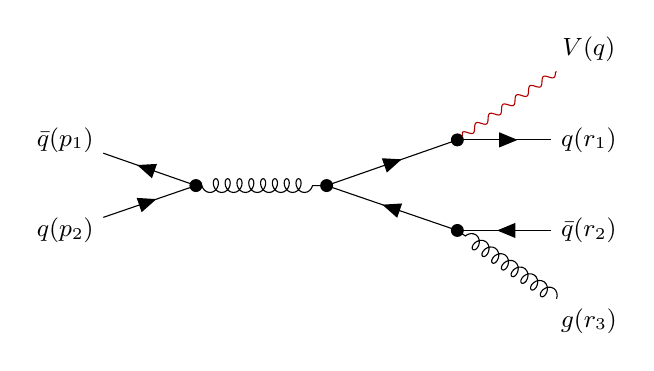
\begin{tikzpicture}[baseline=(current bounding box.center)]
\begin{feynman}
\vertex (e1) at (0.43,2.59) {\small $\bar q(p_1)$};
\vertex (e3) at (0.43,1.44) {\small $q(p_2)$};
\vertex (e5) at (7.08,3.74) {\small $V(q)$};
\vertex (e7) at (7.08,2.59) {\small $q(r_1)$};
\vertex (e9) at (7.08,1.44) {\small $\bar q(r_2)$};
\vertex (e11) at (7.08,0.29) {\small $g(r_3)$};
\vertex[dot] (v0) at (2.09,2.01) {};
\vertex[dot] (v1) at (5.41,2.59) {};
\vertex[dot] (v2) at (5.41,1.44) {};
\vertex[dot] (v3) at (3.75,2.01) {};
\diagram* {
(v0) -- [fermion] (e1),
(e3) -- [fermion] (v0),
(e5) -- [boson, red!70!black] (v1),
(v1) -- [fermion] (e7),
(e9) -- [fermion] (v2),
(e11) -- [gluon] (v2),
(v0) -- [gluon] (v3),
(v3) -- [fermion] (v1),
(v2) -- [fermion] (v3),
};
\end{feynman}
\end{tikzpicture}}\\[2mm]\textbf{Vqbqqqbg}: $\bar q q \to V\, q \bar q g$\\ {\footnotesize diagram 1 of 48, p1$\leftrightarrow$p2 partner Vqqbqqbg}\end{minipage}\hfill%
\begin{minipage}[t]{0.48\textwidth}\centering\resizebox{0.95\linewidth}{!}{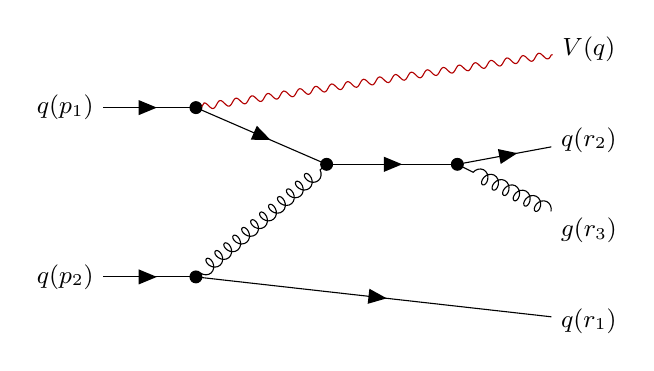
\begin{tikzpicture}[baseline=(current bounding box.center)]
\begin{feynman}
\vertex (e1) at (0.43,3.00) {\small $q(p_1)$};
\vertex (e3) at (0.43,0.85) {\small $q(p_2)$};
\vertex (e5) at (7.08,3.74) {\small $V(q)$};
\vertex (e7) at (7.08,0.29) {\small $q(r_1)$};
\vertex (e9) at (7.08,2.59) {\small $q(r_2)$};
\vertex (e11) at (7.08,1.44) {\small $g(r_3)$};
\vertex[dot] (v0) at (2.09,3.00) {};
\vertex[dot] (v1) at (2.09,0.85) {};
\vertex[dot] (v2) at (5.41,2.28) {};
\vertex[dot] (v3) at (3.75,2.28) {};
\diagram* {
(e1) -- [fermion] (v0),
(e3) -- [fermion] (v1),
(e5) -- [boson, red!70!black] (v0),
(v1) -- [fermion] (e7),
(v2) -- [fermion] (e9),
(e11) -- [gluon] (v2),
(v0) -- [fermion] (v3),
(v1) -- [gluon] (v3),
(v3) -- [fermion] (v2),
};
\end{feynman}
\end{tikzpicture}}\\[2mm]\textbf{Vqqqqg}: $q q \to V\, q q g$\\ {\footnotesize diagram 1 of 48, p1$\leftrightarrow$p2 symmetric}\end{minipage}\hfill

\bigskip

\section*{\texttt{ghosts\_qqbccbg}}
\begin{minipage}[t]{0.48\textwidth}\centering\resizebox{0.95\linewidth}{!}{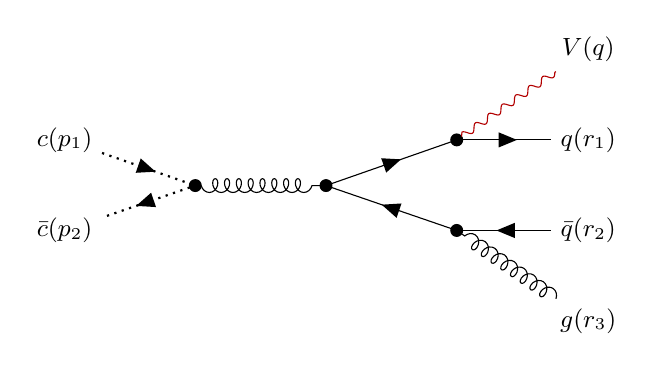
\begin{tikzpicture}[baseline=(current bounding box.center)]
\begin{feynman}
\vertex (e1) at (0.43,2.59) {\small $c(p_1)$};
\vertex (e3) at (0.43,1.44) {\small $\bar c(p_2)$};
\vertex (e5) at (7.08,3.74) {\small $V(q)$};
\vertex (e7) at (7.08,2.59) {\small $q(r_1)$};
\vertex (e9) at (7.08,1.44) {\small $\bar q(r_2)$};
\vertex (e11) at (7.08,0.29) {\small $g(r_3)$};
\vertex[dot] (v0) at (2.09,2.01) {};
\vertex[dot] (v1) at (5.41,2.59) {};
\vertex[dot] (v2) at (5.41,1.44) {};
\vertex[dot] (v3) at (3.75,2.01) {};
\diagram* {
(e1) -- [ghost, with arrow=0.5] (v0),
(v0) -- [ghost, with arrow=0.5] (e3),
(e5) -- [boson, red!70!black] (v1),
(v1) -- [fermion] (e7),
(e9) -- [fermion] (v2),
(e11) -- [gluon] (v2),
(v0) -- [gluon] (v3),
(v3) -- [fermion] (v1),
(v2) -- [fermion] (v3),
};
\end{feynman}
\end{tikzpicture}}\\[2mm]\textbf{Vccbqqbg}: $c \bar c \to V\, q \bar q g$\\ {\footnotesize diagram 1 of 12, p1$\leftrightarrow$p2 partner Vcbcqqbg}\end{minipage}\hfill%
\begin{minipage}[t]{0.48\textwidth}\centering\resizebox{0.95\linewidth}{!}{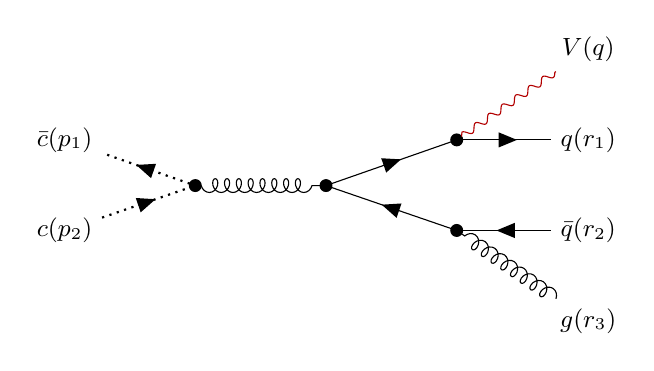
\begin{tikzpicture}[baseline=(current bounding box.center)]
\begin{feynman}
\vertex (e1) at (0.43,2.59) {\small $\bar c(p_1)$};
\vertex (e3) at (0.43,1.44) {\small $c(p_2)$};
\vertex (e5) at (7.08,3.74) {\small $V(q)$};
\vertex (e7) at (7.08,2.59) {\small $q(r_1)$};
\vertex (e9) at (7.08,1.44) {\small $\bar q(r_2)$};
\vertex (e11) at (7.08,0.29) {\small $g(r_3)$};
\vertex[dot] (v0) at (2.09,2.01) {};
\vertex[dot] (v1) at (5.41,2.59) {};
\vertex[dot] (v2) at (5.41,1.44) {};
\vertex[dot] (v3) at (3.75,2.01) {};
\diagram* {
(v0) -- [ghost, with arrow=0.5] (e1),
(e3) -- [ghost, with arrow=0.5] (v0),
(e5) -- [boson, red!70!black] (v1),
(v1) -- [fermion] (e7),
(e9) -- [fermion] (v2),
(e11) -- [gluon] (v2),
(v0) -- [gluon] (v3),
(v3) -- [fermion] (v1),
(v2) -- [fermion] (v3),
};
\end{feynman}
\end{tikzpicture}}\\[2mm]\textbf{Vcbcqqbg}: $\bar c c \to V\, q \bar q g$\\ {\footnotesize diagram 1 of 12, p1$\leftrightarrow$p2 partner Vccbqqbg}\end{minipage}\hfill

\bigskip

\begin{minipage}[t]{0.48\textwidth}\centering\resizebox{0.95\linewidth}{!}{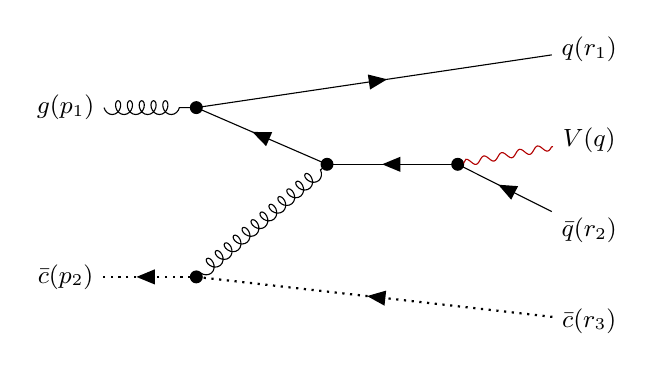
\begin{tikzpicture}[baseline=(current bounding box.center)]
\begin{feynman}
\vertex (e1) at (0.43,3.00) {\small $g(p_1)$};
\vertex (e3) at (0.43,0.85) {\small $\bar c(p_2)$};
\vertex (e5) at (7.08,2.59) {\small $V(q)$};
\vertex (e7) at (7.08,3.74) {\small $q(r_1)$};
\vertex (e9) at (7.08,1.44) {\small $\bar q(r_2)$};
\vertex (e11) at (7.08,0.29) {\small $\bar c(r_3)$};
\vertex[dot] (v0) at (2.09,3.00) {};
\vertex[dot] (v1) at (2.09,0.85) {};
\vertex[dot] (v2) at (5.41,2.28) {};
\vertex[dot] (v3) at (3.75,2.28) {};
\diagram* {
(e1) -- [gluon] (v0),
(v1) -- [ghost, with arrow=0.5] (e3),
(e5) -- [boson, red!70!black] (v2),
(v0) -- [fermion] (e7),
(e9) -- [fermion] (v2),
(e11) -- [ghost, with arrow=0.5] (v1),
(v3) -- [fermion] (v0),
(v1) -- [gluon] (v3),
(v2) -- [fermion] (v3),
};
\end{feynman}
\end{tikzpicture}}\\[2mm]\textbf{Vgcbqqbcb}: $g \bar c \to V\, q \bar q \bar c$\\ {\footnotesize diagram 1 of 12, p1$\leftrightarrow$p2 partner Vcbgqqbcb}\end{minipage}\hfill%
\begin{minipage}[t]{0.48\textwidth}\centering\resizebox{0.95\linewidth}{!}{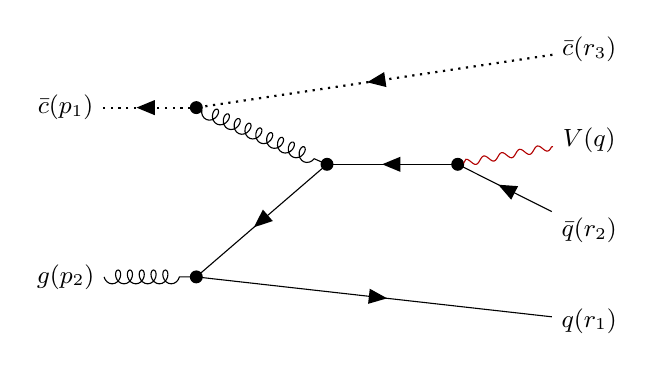
\begin{tikzpicture}[baseline=(current bounding box.center)]
\begin{feynman}
\vertex (e1) at (0.43,3.00) {\small $\bar c(p_1)$};
\vertex (e3) at (0.43,0.85) {\small $g(p_2)$};
\vertex (e5) at (7.08,2.59) {\small $V(q)$};
\vertex (e7) at (7.08,0.29) {\small $q(r_1)$};
\vertex (e9) at (7.08,1.44) {\small $\bar q(r_2)$};
\vertex (e11) at (7.08,3.74) {\small $\bar c(r_3)$};
\vertex[dot] (v0) at (2.09,3.00) {};
\vertex[dot] (v1) at (2.09,0.85) {};
\vertex[dot] (v2) at (5.41,2.28) {};
\vertex[dot] (v3) at (3.75,2.28) {};
\diagram* {
(v0) -- [ghost, with arrow=0.5] (e1),
(e3) -- [gluon] (v1),
(e5) -- [boson, red!70!black] (v2),
(v1) -- [fermion] (e7),
(e9) -- [fermion] (v2),
(e11) -- [ghost, with arrow=0.5] (v0),
(v0) -- [gluon] (v3),
(v3) -- [fermion] (v1),
(v2) -- [fermion] (v3),
};
\end{feynman}
\end{tikzpicture}}\\[2mm]\textbf{Vcbgqqbcb}: $\bar c g \to V\, q \bar q \bar c$\\ {\footnotesize diagram 1 of 12, p1$\leftrightarrow$p2 partner Vgcbqqbcb}\end{minipage}\hfill

\bigskip

\begin{minipage}[t]{0.48\textwidth}\centering\resizebox{0.95\linewidth}{!}{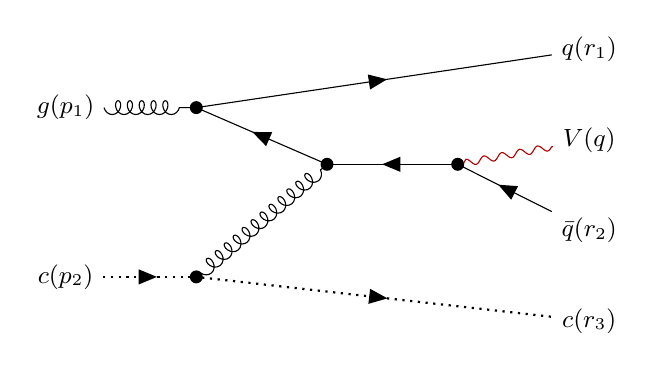
\begin{tikzpicture}[baseline=(current bounding box.center)]
\begin{feynman}
\vertex (e1) at (0.43,3.00) {\small $g(p_1)$};
\vertex (e3) at (0.43,0.85) {\small $c(p_2)$};
\vertex (e5) at (7.08,2.59) {\small $V(q)$};
\vertex (e7) at (7.08,3.74) {\small $q(r_1)$};
\vertex (e9) at (7.08,1.44) {\small $\bar q(r_2)$};
\vertex (e11) at (7.08,0.29) {\small $c(r_3)$};
\vertex[dot] (v0) at (2.09,3.00) {};
\vertex[dot] (v1) at (2.09,0.85) {};
\vertex[dot] (v2) at (5.41,2.28) {};
\vertex[dot] (v3) at (3.75,2.28) {};
\diagram* {
(e1) -- [gluon] (v0),
(e3) -- [ghost, with arrow=0.5] (v1),
(e5) -- [boson, red!70!black] (v2),
(v0) -- [fermion] (e7),
(e9) -- [fermion] (v2),
(v1) -- [ghost, with arrow=0.5] (e11),
(v3) -- [fermion] (v0),
(v1) -- [gluon] (v3),
(v2) -- [fermion] (v3),
};
\end{feynman}
\end{tikzpicture}}\\[2mm]\textbf{Vgcqqbc}: $g c \to V\, q \bar q c$\\ {\footnotesize diagram 1 of 12, p1$\leftrightarrow$p2 partner Vcgqqbc}\end{minipage}\hfill%
\begin{minipage}[t]{0.48\textwidth}\centering\resizebox{0.95\linewidth}{!}{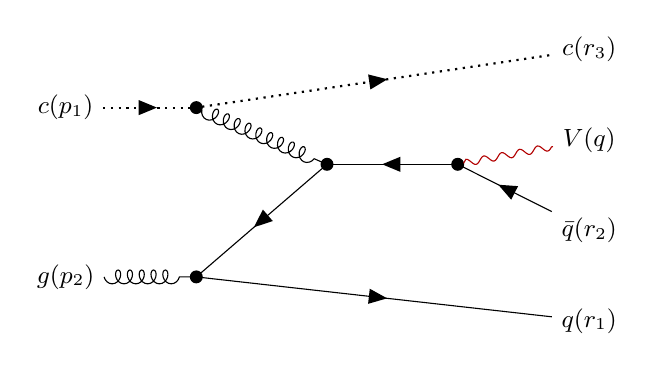
\begin{tikzpicture}[baseline=(current bounding box.center)]
\begin{feynman}
\vertex (e1) at (0.43,3.00) {\small $c(p_1)$};
\vertex (e3) at (0.43,0.85) {\small $g(p_2)$};
\vertex (e5) at (7.08,2.59) {\small $V(q)$};
\vertex (e7) at (7.08,0.29) {\small $q(r_1)$};
\vertex (e9) at (7.08,1.44) {\small $\bar q(r_2)$};
\vertex (e11) at (7.08,3.74) {\small $c(r_3)$};
\vertex[dot] (v0) at (2.09,3.00) {};
\vertex[dot] (v1) at (2.09,0.85) {};
\vertex[dot] (v2) at (5.41,2.28) {};
\vertex[dot] (v3) at (3.75,2.28) {};
\diagram* {
(e1) -- [ghost, with arrow=0.5] (v0),
(e3) -- [gluon] (v1),
(e5) -- [boson, red!70!black] (v2),
(v1) -- [fermion] (e7),
(e9) -- [fermion] (v2),
(v0) -- [ghost, with arrow=0.5] (e11),
(v0) -- [gluon] (v3),
(v3) -- [fermion] (v1),
(v2) -- [fermion] (v3),
};
\end{feynman}
\end{tikzpicture}}\\[2mm]\textbf{Vcgqqbc}: $c g \to V\, q \bar q c$\\ {\footnotesize diagram 1 of 12, p1$\leftrightarrow$p2 partner Vgcqqbc}\end{minipage}\hfill

\bigskip

\begin{minipage}[t]{0.48\textwidth}\centering\resizebox{0.95\linewidth}{!}{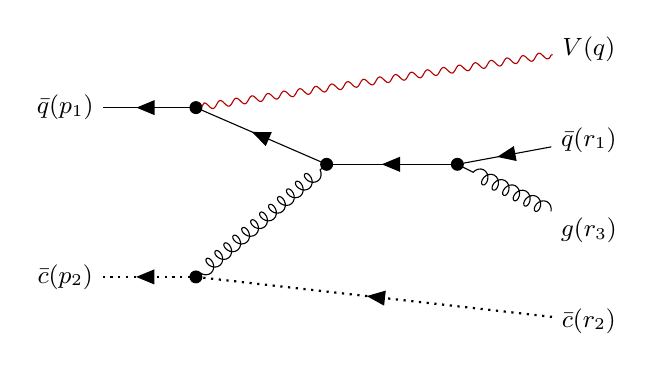
\begin{tikzpicture}[baseline=(current bounding box.center)]
\begin{feynman}
\vertex (e1) at (0.43,3.00) {\small $\bar q(p_1)$};
\vertex (e3) at (0.43,0.85) {\small $\bar c(p_2)$};
\vertex (e5) at (7.08,3.74) {\small $V(q)$};
\vertex (e7) at (7.08,2.59) {\small $\bar q(r_1)$};
\vertex (e9) at (7.08,0.29) {\small $\bar c(r_2)$};
\vertex (e11) at (7.08,1.44) {\small $g(r_3)$};
\vertex[dot] (v0) at (2.09,3.00) {};
\vertex[dot] (v1) at (2.09,0.85) {};
\vertex[dot] (v2) at (5.41,2.28) {};
\vertex[dot] (v3) at (3.75,2.28) {};
\diagram* {
(v0) -- [fermion] (e1),
(v1) -- [ghost, with arrow=0.5] (e3),
(e5) -- [boson, red!70!black] (v0),
(e7) -- [fermion] (v2),
(e9) -- [ghost, with arrow=0.5] (v1),
(e11) -- [gluon] (v2),
(v3) -- [fermion] (v0),
(v1) -- [gluon] (v3),
(v2) -- [fermion] (v3),
};
\end{feynman}
\end{tikzpicture}}\\[2mm]\textbf{Vqbcbqbcbg}: $\bar q \bar c \to V\, \bar q \bar c g$\\ {\footnotesize diagram 1 of 12, p1$\leftrightarrow$p2 partner Vcbqbqbcbg}\end{minipage}\hfill%
\begin{minipage}[t]{0.48\textwidth}\centering\resizebox{0.95\linewidth}{!}{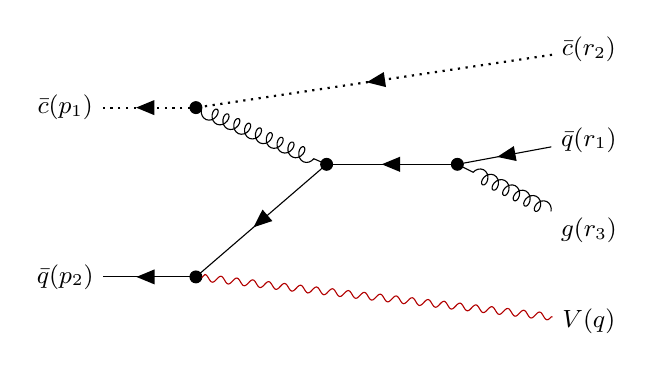
\begin{tikzpicture}[baseline=(current bounding box.center)]
\begin{feynman}
\vertex (e1) at (0.43,3.00) {\small $\bar c(p_1)$};
\vertex (e3) at (0.43,0.85) {\small $\bar q(p_2)$};
\vertex (e5) at (7.08,0.29) {\small $V(q)$};
\vertex (e7) at (7.08,2.59) {\small $\bar q(r_1)$};
\vertex (e9) at (7.08,3.74) {\small $\bar c(r_2)$};
\vertex (e11) at (7.08,1.44) {\small $g(r_3)$};
\vertex[dot] (v0) at (2.09,3.00) {};
\vertex[dot] (v1) at (2.09,0.85) {};
\vertex[dot] (v2) at (5.41,2.28) {};
\vertex[dot] (v3) at (3.75,2.28) {};
\diagram* {
(v0) -- [ghost, with arrow=0.5] (e1),
(v1) -- [fermion] (e3),
(e5) -- [boson, red!70!black] (v1),
(e7) -- [fermion] (v2),
(e9) -- [ghost, with arrow=0.5] (v0),
(e11) -- [gluon] (v2),
(v0) -- [gluon] (v3),
(v3) -- [fermion] (v1),
(v2) -- [fermion] (v3),
};
\end{feynman}
\end{tikzpicture}}\\[2mm]\textbf{Vcbqbqbcbg}: $\bar c \bar q \to V\, \bar q \bar c g$\\ {\footnotesize diagram 1 of 12, p1$\leftrightarrow$p2 partner Vqbcbqbcbg}\end{minipage}\hfill

\bigskip

\begin{minipage}[t]{0.48\textwidth}\centering\resizebox{0.95\linewidth}{!}{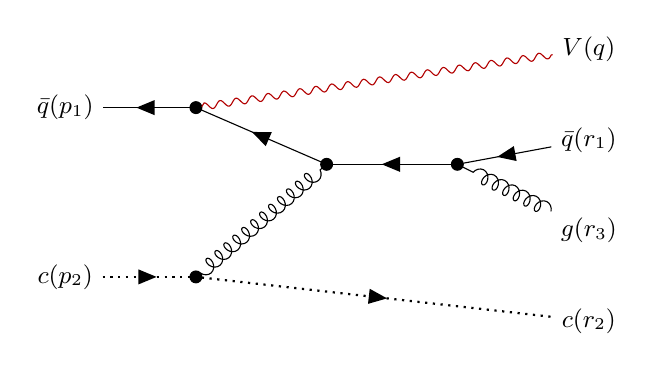
\begin{tikzpicture}[baseline=(current bounding box.center)]
\begin{feynman}
\vertex (e1) at (0.43,3.00) {\small $\bar q(p_1)$};
\vertex (e3) at (0.43,0.85) {\small $c(p_2)$};
\vertex (e5) at (7.08,3.74) {\small $V(q)$};
\vertex (e7) at (7.08,2.59) {\small $\bar q(r_1)$};
\vertex (e9) at (7.08,0.29) {\small $c(r_2)$};
\vertex (e11) at (7.08,1.44) {\small $g(r_3)$};
\vertex[dot] (v0) at (2.09,3.00) {};
\vertex[dot] (v1) at (2.09,0.85) {};
\vertex[dot] (v2) at (5.41,2.28) {};
\vertex[dot] (v3) at (3.75,2.28) {};
\diagram* {
(v0) -- [fermion] (e1),
(e3) -- [ghost, with arrow=0.5] (v1),
(e5) -- [boson, red!70!black] (v0),
(e7) -- [fermion] (v2),
(v1) -- [ghost, with arrow=0.5] (e9),
(e11) -- [gluon] (v2),
(v3) -- [fermion] (v0),
(v1) -- [gluon] (v3),
(v2) -- [fermion] (v3),
};
\end{feynman}
\end{tikzpicture}}\\[2mm]\textbf{Vqbcqbcg}: $\bar q c \to V\, \bar q c g$\\ {\footnotesize diagram 1 of 12, p1$\leftrightarrow$p2 partner Vcqbqbcg}\end{minipage}\hfill%
\begin{minipage}[t]{0.48\textwidth}\centering\resizebox{0.95\linewidth}{!}{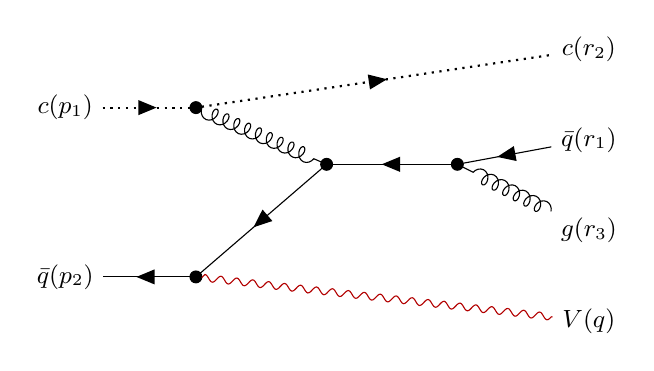
\begin{tikzpicture}[baseline=(current bounding box.center)]
\begin{feynman}
\vertex (e1) at (0.43,3.00) {\small $c(p_1)$};
\vertex (e3) at (0.43,0.85) {\small $\bar q(p_2)$};
\vertex (e5) at (7.08,0.29) {\small $V(q)$};
\vertex (e7) at (7.08,2.59) {\small $\bar q(r_1)$};
\vertex (e9) at (7.08,3.74) {\small $c(r_2)$};
\vertex (e11) at (7.08,1.44) {\small $g(r_3)$};
\vertex[dot] (v0) at (2.09,3.00) {};
\vertex[dot] (v1) at (2.09,0.85) {};
\vertex[dot] (v2) at (5.41,2.28) {};
\vertex[dot] (v3) at (3.75,2.28) {};
\diagram* {
(e1) -- [ghost, with arrow=0.5] (v0),
(v1) -- [fermion] (e3),
(e5) -- [boson, red!70!black] (v1),
(e7) -- [fermion] (v2),
(v0) -- [ghost, with arrow=0.5] (e9),
(e11) -- [gluon] (v2),
(v0) -- [gluon] (v3),
(v3) -- [fermion] (v1),
(v2) -- [fermion] (v3),
};
\end{feynman}
\end{tikzpicture}}\\[2mm]\textbf{Vcqbqbcg}: $c \bar q \to V\, \bar q c g$\\ {\footnotesize diagram 1 of 12, p1$\leftrightarrow$p2 partner Vqbcqbcg}\end{minipage}\hfill

\bigskip

\begin{minipage}[t]{0.48\textwidth}\centering\resizebox{0.95\linewidth}{!}{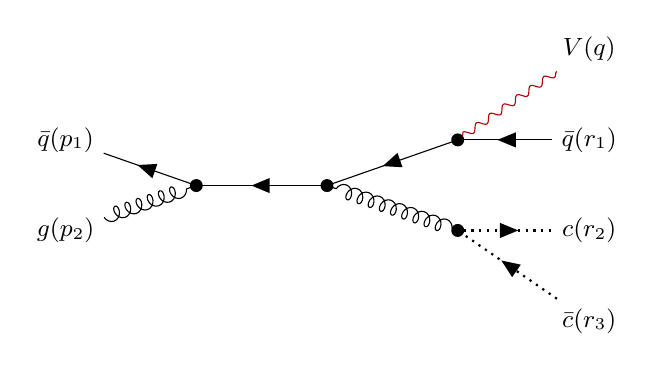
\begin{tikzpicture}[baseline=(current bounding box.center)]
\begin{feynman}
\vertex (e1) at (0.43,2.59) {\small $\bar q(p_1)$};
\vertex (e3) at (0.43,1.44) {\small $g(p_2)$};
\vertex (e5) at (7.08,3.74) {\small $V(q)$};
\vertex (e7) at (7.08,2.59) {\small $\bar q(r_1)$};
\vertex (e9) at (7.08,1.44) {\small $c(r_2)$};
\vertex (e11) at (7.08,0.29) {\small $\bar c(r_3)$};
\vertex[dot] (v0) at (2.09,2.01) {};
\vertex[dot] (v1) at (5.41,2.59) {};
\vertex[dot] (v2) at (5.41,1.44) {};
\vertex[dot] (v3) at (3.75,2.01) {};
\diagram* {
(v0) -- [fermion] (e1),
(e3) -- [gluon] (v0),
(e5) -- [boson, red!70!black] (v1),
(e7) -- [fermion] (v1),
(v2) -- [ghost, with arrow=0.5] (e9),
(e11) -- [ghost, with arrow=0.5] (v2),
(v3) -- [fermion] (v0),
(v1) -- [fermion] (v3),
(v2) -- [gluon] (v3),
};
\end{feynman}
\end{tikzpicture}}\\[2mm]\textbf{Vqbgqbccb}: $\bar q g \to V\, \bar q c \bar c$\\ {\footnotesize diagram 1 of 12, p1$\leftrightarrow$p2 partner Vgqbqbccb}\end{minipage}\hfill%
\begin{minipage}[t]{0.48\textwidth}\centering\resizebox{0.95\linewidth}{!}{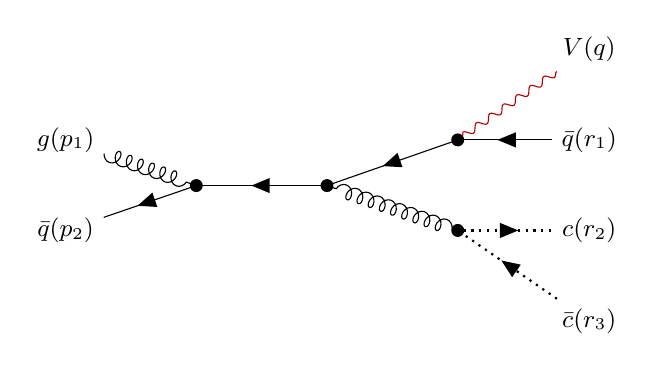
\begin{tikzpicture}[baseline=(current bounding box.center)]
\begin{feynman}
\vertex (e1) at (0.43,2.59) {\small $g(p_1)$};
\vertex (e3) at (0.43,1.44) {\small $\bar q(p_2)$};
\vertex (e5) at (7.08,3.74) {\small $V(q)$};
\vertex (e7) at (7.08,2.59) {\small $\bar q(r_1)$};
\vertex (e9) at (7.08,1.44) {\small $c(r_2)$};
\vertex (e11) at (7.08,0.29) {\small $\bar c(r_3)$};
\vertex[dot] (v0) at (2.09,2.01) {};
\vertex[dot] (v1) at (5.41,2.59) {};
\vertex[dot] (v2) at (5.41,1.44) {};
\vertex[dot] (v3) at (3.75,2.01) {};
\diagram* {
(e1) -- [gluon] (v0),
(v0) -- [fermion] (e3),
(e5) -- [boson, red!70!black] (v1),
(e7) -- [fermion] (v1),
(v2) -- [ghost, with arrow=0.5] (e9),
(e11) -- [ghost, with arrow=0.5] (v2),
(v3) -- [fermion] (v0),
(v1) -- [fermion] (v3),
(v2) -- [gluon] (v3),
};
\end{feynman}
\end{tikzpicture}}\\[2mm]\textbf{Vgqbqbccb}: $g \bar q \to V\, \bar q c \bar c$\\ {\footnotesize diagram 1 of 12, p1$\leftrightarrow$p2 partner Vqbgqbccb}\end{minipage}\hfill

\bigskip

\begin{minipage}[t]{0.48\textwidth}\centering\resizebox{0.95\linewidth}{!}{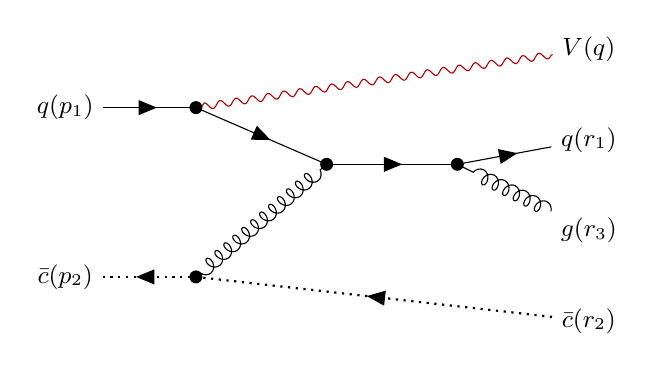
\begin{tikzpicture}[baseline=(current bounding box.center)]
\begin{feynman}
\vertex (e1) at (0.43,3.00) {\small $q(p_1)$};
\vertex (e3) at (0.43,0.85) {\small $\bar c(p_2)$};
\vertex (e5) at (7.08,3.74) {\small $V(q)$};
\vertex (e7) at (7.08,2.59) {\small $q(r_1)$};
\vertex (e9) at (7.08,0.29) {\small $\bar c(r_2)$};
\vertex (e11) at (7.08,1.44) {\small $g(r_3)$};
\vertex[dot] (v0) at (2.09,3.00) {};
\vertex[dot] (v1) at (2.09,0.85) {};
\vertex[dot] (v2) at (5.41,2.28) {};
\vertex[dot] (v3) at (3.75,2.28) {};
\diagram* {
(e1) -- [fermion] (v0),
(v1) -- [ghost, with arrow=0.5] (e3),
(e5) -- [boson, red!70!black] (v0),
(v2) -- [fermion] (e7),
(e9) -- [ghost, with arrow=0.5] (v1),
(e11) -- [gluon] (v2),
(v0) -- [fermion] (v3),
(v1) -- [gluon] (v3),
(v3) -- [fermion] (v2),
};
\end{feynman}
\end{tikzpicture}}\\[2mm]\textbf{Vqcbqcbg}: $q \bar c \to V\, q \bar c g$\\ {\footnotesize diagram 1 of 12, p1$\leftrightarrow$p2 partner Vcbqqcbg}\end{minipage}\hfill%
\begin{minipage}[t]{0.48\textwidth}\centering\resizebox{0.95\linewidth}{!}{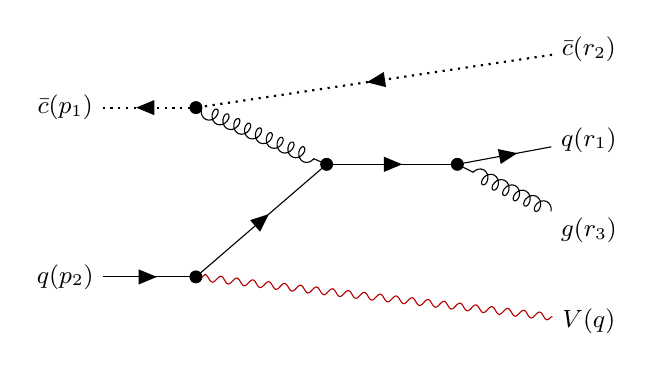
\begin{tikzpicture}[baseline=(current bounding box.center)]
\begin{feynman}
\vertex (e1) at (0.43,3.00) {\small $\bar c(p_1)$};
\vertex (e3) at (0.43,0.85) {\small $q(p_2)$};
\vertex (e5) at (7.08,0.29) {\small $V(q)$};
\vertex (e7) at (7.08,2.59) {\small $q(r_1)$};
\vertex (e9) at (7.08,3.74) {\small $\bar c(r_2)$};
\vertex (e11) at (7.08,1.44) {\small $g(r_3)$};
\vertex[dot] (v0) at (2.09,3.00) {};
\vertex[dot] (v1) at (2.09,0.85) {};
\vertex[dot] (v2) at (5.41,2.28) {};
\vertex[dot] (v3) at (3.75,2.28) {};
\diagram* {
(v0) -- [ghost, with arrow=0.5] (e1),
(e3) -- [fermion] (v1),
(e5) -- [boson, red!70!black] (v1),
(v2) -- [fermion] (e7),
(e9) -- [ghost, with arrow=0.5] (v0),
(e11) -- [gluon] (v2),
(v0) -- [gluon] (v3),
(v1) -- [fermion] (v3),
(v3) -- [fermion] (v2),
};
\end{feynman}
\end{tikzpicture}}\\[2mm]\textbf{Vcbqqcbg}: $\bar c q \to V\, q \bar c g$\\ {\footnotesize diagram 1 of 12, p1$\leftrightarrow$p2 partner Vqcbqcbg}\end{minipage}\hfill

\bigskip

\begin{minipage}[t]{0.48\textwidth}\centering\resizebox{0.95\linewidth}{!}{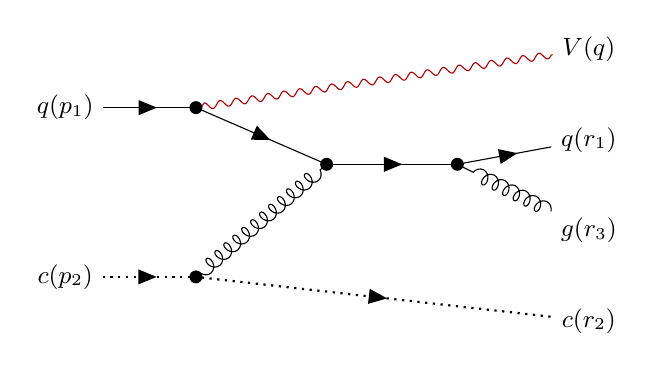
\begin{tikzpicture}[baseline=(current bounding box.center)]
\begin{feynman}
\vertex (e1) at (0.43,3.00) {\small $q(p_1)$};
\vertex (e3) at (0.43,0.85) {\small $c(p_2)$};
\vertex (e5) at (7.08,3.74) {\small $V(q)$};
\vertex (e7) at (7.08,2.59) {\small $q(r_1)$};
\vertex (e9) at (7.08,0.29) {\small $c(r_2)$};
\vertex (e11) at (7.08,1.44) {\small $g(r_3)$};
\vertex[dot] (v0) at (2.09,3.00) {};
\vertex[dot] (v1) at (2.09,0.85) {};
\vertex[dot] (v2) at (5.41,2.28) {};
\vertex[dot] (v3) at (3.75,2.28) {};
\diagram* {
(e1) -- [fermion] (v0),
(e3) -- [ghost, with arrow=0.5] (v1),
(e5) -- [boson, red!70!black] (v0),
(v2) -- [fermion] (e7),
(v1) -- [ghost, with arrow=0.5] (e9),
(e11) -- [gluon] (v2),
(v0) -- [fermion] (v3),
(v1) -- [gluon] (v3),
(v3) -- [fermion] (v2),
};
\end{feynman}
\end{tikzpicture}}\\[2mm]\textbf{Vqcqcg}: $q c \to V\, q c g$\\ {\footnotesize diagram 1 of 12, p1$\leftrightarrow$p2 partner Vcqqcg}\end{minipage}\hfill%
\begin{minipage}[t]{0.48\textwidth}\centering\resizebox{0.95\linewidth}{!}{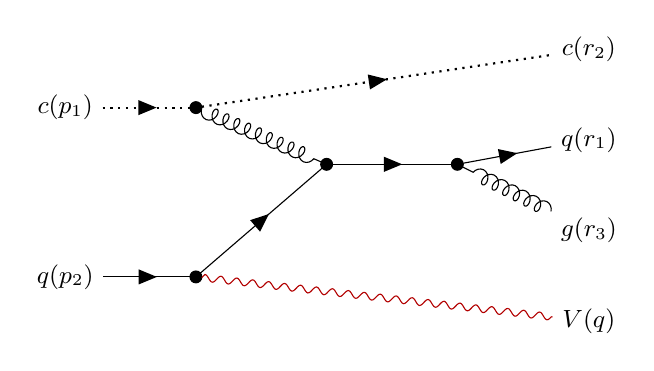
\begin{tikzpicture}[baseline=(current bounding box.center)]
\begin{feynman}
\vertex (e1) at (0.43,3.00) {\small $c(p_1)$};
\vertex (e3) at (0.43,0.85) {\small $q(p_2)$};
\vertex (e5) at (7.08,0.29) {\small $V(q)$};
\vertex (e7) at (7.08,2.59) {\small $q(r_1)$};
\vertex (e9) at (7.08,3.74) {\small $c(r_2)$};
\vertex (e11) at (7.08,1.44) {\small $g(r_3)$};
\vertex[dot] (v0) at (2.09,3.00) {};
\vertex[dot] (v1) at (2.09,0.85) {};
\vertex[dot] (v2) at (5.41,2.28) {};
\vertex[dot] (v3) at (3.75,2.28) {};
\diagram* {
(e1) -- [ghost, with arrow=0.5] (v0),
(e3) -- [fermion] (v1),
(e5) -- [boson, red!70!black] (v1),
(v2) -- [fermion] (e7),
(v0) -- [ghost, with arrow=0.5] (e9),
(e11) -- [gluon] (v2),
(v0) -- [gluon] (v3),
(v1) -- [fermion] (v3),
(v3) -- [fermion] (v2),
};
\end{feynman}
\end{tikzpicture}}\\[2mm]\textbf{Vcqqcg}: $c q \to V\, q c g$\\ {\footnotesize diagram 1 of 12, p1$\leftrightarrow$p2 partner Vqcqcg}\end{minipage}\hfill

\bigskip

\begin{minipage}[t]{0.48\textwidth}\centering\resizebox{0.95\linewidth}{!}{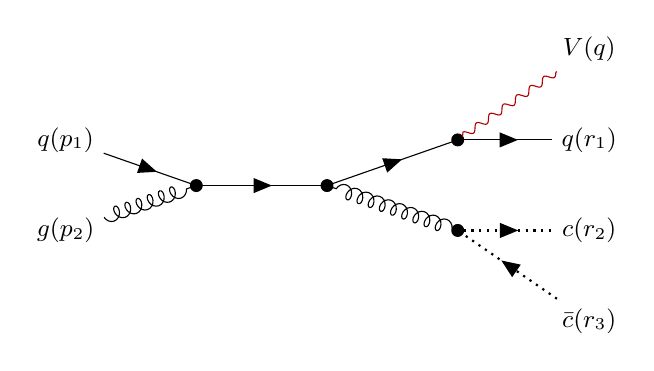
\begin{tikzpicture}[baseline=(current bounding box.center)]
\begin{feynman}
\vertex (e1) at (0.43,2.59) {\small $q(p_1)$};
\vertex (e3) at (0.43,1.44) {\small $g(p_2)$};
\vertex (e5) at (7.08,3.74) {\small $V(q)$};
\vertex (e7) at (7.08,2.59) {\small $q(r_1)$};
\vertex (e9) at (7.08,1.44) {\small $c(r_2)$};
\vertex (e11) at (7.08,0.29) {\small $\bar c(r_3)$};
\vertex[dot] (v0) at (2.09,2.01) {};
\vertex[dot] (v1) at (5.41,2.59) {};
\vertex[dot] (v2) at (5.41,1.44) {};
\vertex[dot] (v3) at (3.75,2.01) {};
\diagram* {
(e1) -- [fermion] (v0),
(e3) -- [gluon] (v0),
(e5) -- [boson, red!70!black] (v1),
(v1) -- [fermion] (e7),
(v2) -- [ghost, with arrow=0.5] (e9),
(e11) -- [ghost, with arrow=0.5] (v2),
(v0) -- [fermion] (v3),
(v3) -- [fermion] (v1),
(v2) -- [gluon] (v3),
};
\end{feynman}
\end{tikzpicture}}\\[2mm]\textbf{Vqgqccb}: $q g \to V\, q c \bar c$\\ {\footnotesize diagram 1 of 12, p1$\leftrightarrow$p2 partner Vgqqccb}\end{minipage}\hfill%
\begin{minipage}[t]{0.48\textwidth}\centering\resizebox{0.95\linewidth}{!}{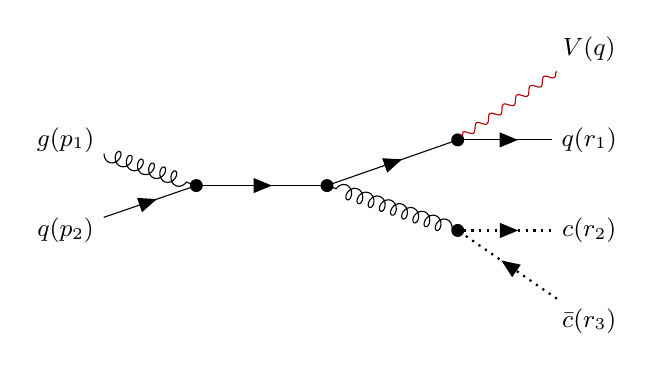
\begin{tikzpicture}[baseline=(current bounding box.center)]
\begin{feynman}
\vertex (e1) at (0.43,2.59) {\small $g(p_1)$};
\vertex (e3) at (0.43,1.44) {\small $q(p_2)$};
\vertex (e5) at (7.08,3.74) {\small $V(q)$};
\vertex (e7) at (7.08,2.59) {\small $q(r_1)$};
\vertex (e9) at (7.08,1.44) {\small $c(r_2)$};
\vertex (e11) at (7.08,0.29) {\small $\bar c(r_3)$};
\vertex[dot] (v0) at (2.09,2.01) {};
\vertex[dot] (v1) at (5.41,2.59) {};
\vertex[dot] (v2) at (5.41,1.44) {};
\vertex[dot] (v3) at (3.75,2.01) {};
\diagram* {
(e1) -- [gluon] (v0),
(e3) -- [fermion] (v0),
(e5) -- [boson, red!70!black] (v1),
(v1) -- [fermion] (e7),
(v2) -- [ghost, with arrow=0.5] (e9),
(e11) -- [ghost, with arrow=0.5] (v2),
(v0) -- [fermion] (v3),
(v3) -- [fermion] (v1),
(v2) -- [gluon] (v3),
};
\end{feynman}
\end{tikzpicture}}\\[2mm]\textbf{Vgqqccb}: $g q \to V\, q c \bar c$\\ {\footnotesize diagram 1 of 12, p1$\leftrightarrow$p2 partner Vqgqccb}\end{minipage}\hfill

\bigskip

\begin{minipage}[t]{0.48\textwidth}\centering\resizebox{0.95\linewidth}{!}{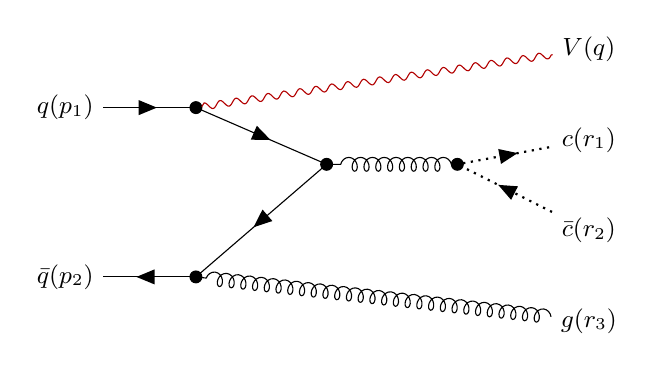
\begin{tikzpicture}[baseline=(current bounding box.center)]
\begin{feynman}
\vertex (e1) at (0.43,3.00) {\small $q(p_1)$};
\vertex (e3) at (0.43,0.85) {\small $\bar q(p_2)$};
\vertex (e5) at (7.08,3.74) {\small $V(q)$};
\vertex (e7) at (7.08,2.59) {\small $c(r_1)$};
\vertex (e9) at (7.08,1.44) {\small $\bar c(r_2)$};
\vertex (e11) at (7.08,0.29) {\small $g(r_3)$};
\vertex[dot] (v0) at (2.09,3.00) {};
\vertex[dot] (v1) at (2.09,0.85) {};
\vertex[dot] (v2) at (5.41,2.28) {};
\vertex[dot] (v3) at (3.75,2.28) {};
\diagram* {
(e1) -- [fermion] (v0),
(v1) -- [fermion] (e3),
(e5) -- [boson, red!70!black] (v0),
(v2) -- [ghost, with arrow=0.5] (e7),
(e9) -- [ghost, with arrow=0.5] (v2),
(e11) -- [gluon] (v1),
(v0) -- [fermion] (v3),
(v3) -- [fermion] (v1),
(v2) -- [gluon] (v3),
};
\end{feynman}
\end{tikzpicture}}\\[2mm]\textbf{Vqqbccbg}: $q \bar q \to V\, c \bar c g$\\ {\footnotesize diagram 1 of 12, p1$\leftrightarrow$p2 partner Vqbqccbg}\end{minipage}\hfill%
\begin{minipage}[t]{0.48\textwidth}\centering\resizebox{0.95\linewidth}{!}{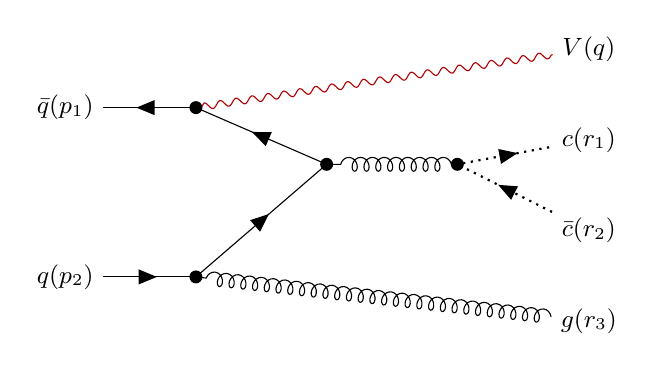
\begin{tikzpicture}[baseline=(current bounding box.center)]
\begin{feynman}
\vertex (e1) at (0.43,3.00) {\small $\bar q(p_1)$};
\vertex (e3) at (0.43,0.85) {\small $q(p_2)$};
\vertex (e5) at (7.08,3.74) {\small $V(q)$};
\vertex (e7) at (7.08,2.59) {\small $c(r_1)$};
\vertex (e9) at (7.08,1.44) {\small $\bar c(r_2)$};
\vertex (e11) at (7.08,0.29) {\small $g(r_3)$};
\vertex[dot] (v0) at (2.09,3.00) {};
\vertex[dot] (v1) at (2.09,0.85) {};
\vertex[dot] (v2) at (5.41,2.28) {};
\vertex[dot] (v3) at (3.75,2.28) {};
\diagram* {
(v0) -- [fermion] (e1),
(e3) -- [fermion] (v1),
(e5) -- [boson, red!70!black] (v0),
(v2) -- [ghost, with arrow=0.5] (e7),
(e9) -- [ghost, with arrow=0.5] (v2),
(e11) -- [gluon] (v1),
(v3) -- [fermion] (v0),
(v1) -- [fermion] (v3),
(v2) -- [gluon] (v3),
};
\end{feynman}
\end{tikzpicture}}\\[2mm]\textbf{Vqbqccbg}: $\bar q q \to V\, c \bar c g$\\ {\footnotesize diagram 1 of 12, p1$\leftrightarrow$p2 partner Vqqbccbg}\end{minipage}\hfill

\bigskip

\end{document}